\documentclass[11pt,a4paper]{article}

\usepackage[utf8]{inputenc}
\usepackage[T1]{fontenc}
\usepackage{lmodern}
\usepackage[margin=1in]{geometry}
\usepackage{amsmath,amssymb}
\usepackage{booktabs}
% boxed names for interactive UI controls (buttons, fields)
\newcommand{\ui}[1]{{\setlength{\fboxsep}{2pt}\fbox{\footnotesize\textsf{#1}}}}
\usepackage{longtable}
\usepackage{array}
\usepackage[dvipsnames]{xcolor}
\usepackage{hyperref}
\usepackage{graphicx}
\usepackage{microtype}
\usepackage{parskip}
\usepackage{enumitem}
\usepackage{fancyvrb}
\usepackage{fancyhdr}
\usepackage{ragged2e}

\hypersetup{
  colorlinks=true,
  linkcolor=blue!60!black,
  citecolor=blue!60!black,
  urlcolor=blue!60!black,
}

% Header/footer
\pagestyle{fancy}
\fancyhf{}
\fancyhead[L]{\small Open Spectrograph: An Aberration-Corrected Fiber-Coupled Czerny-Turner Spectrograph}
\fancyfoot[L]{\small \textcopyright\ 2026. Licensed under \href{https://ohwr.org/cern_ohl_p_v2.txt}{CERN-OHL-P v2} (hardware) and \href{https://opensource.org/licenses/MIT}{MIT} (software).}
\fancyfoot[R]{\thepage}
\renewcommand{\headrulewidth}{0.4pt}
\renewcommand{\footrulewidth}{0.4pt}

% Git version info (auto-generated by build_paper.sh)
\IfFileExists{version.tex}{\input{version}}{%
  \newcommand{\gitversion}{dev}%
  \newcommand{\gitdate}{\today}}

\begin{document}

\begin{titlepage}
\centering
\vspace*{2cm}
{\Huge\bfseries Open Spectrograph}\\[1cm]
{\Large An Aberration-Corrected Fiber-Coupled\\Czerny-Turner Spectrograph}\\[0.5cm]
{\large \gitdate}\\[0.3cm]
{\small Version \gitversion}\\[1.5cm]
\begin{minipage}{0.85\textwidth}
\centering\textbf{Abstract}\\[0.5em]
\justify
We present an aberration-corrected fiber-coupled Czerny-Turner
spectrograph achieving sub-1\,nm spectral resolution over 400--700\,nm
at $f/4$. Built from off-the-shelf catalog optics, 3D-printed flexure
mounts, and an open-source 16-bit linear CCD detector, the complete
instrument targets a bill of materials under \$500, less than a quarter
of comparable commercial spectrometers. The design is driven by a
non-sequential ray-tracing pipeline validated against published Zemax
results. A genetic algorithm built around the ray tracer evolves the
optical geometry, scoring each candidate for spot size and throughput;
a procedural generator then produces the flexure mounts and housing
directly from the winning geometry, ready to 3D-print and assemble.
\end{minipage}
\vfill
{\small \textit{Open Spectrograph: An Aberration-Corrected Fiber-Coupled Czerny-Turner Spectrograph}\\ \textcopyright\ 2026. Licensed under \href{https://ohwr.org/cern_ohl_p_v2.txt}{CERN-OHL-P v2} (hardware) and \href{https://opensource.org/licenses/MIT}{MIT} (software).}
\end{titlepage}
\newpage

\newpage
\tableofcontents
\newpage

%% ===================================================================
\section{Introduction}
%% ===================================================================

\textit{We identify the gap between commercial miniature spectrometers
and existing open-source efforts, and describe a simulation-driven
approach that bridges optical design to fabrication-ready output in a
single toolchain.}

\subsection{The miniature spectrometer landscape}

Compact fiber-coupled spectrometers have become ubiquitous tools in
analytical spectroscopy. Since Ocean Optics (now Ocean Insight)
introduced the first miniature fiber spectrometer S1000 in 1992, the
market has
consolidated around a common architecture: a Czerny-Turner optical
train with a fixed diffraction grating and a linear CCD or CMOS
detector array, packaged in a machined aluminum enclosure roughly the
size of a deck of cards. The leading commercial instruments are
summarized in Table~\ref{tab:commercial}.

\begin{table}[h]
\centering
\caption{Leading commercial miniature fiber spectrometers.}
\label{tab:commercial}
\begin{tabular*}{\textwidth}{@{\extracolsep{\fill}}llp{7.5cm}@{}}
\toprule
Manufacturer & Model(s) & Notes \\
\midrule
Ocean Insight & USB4000, Flame, HDX &
  USB4000 (discontinued) established the sub-\$3000 baseline:
  TCD1304 CCD, 200--1100\,nm, $\sim$1.5\,nm FWHM\@. Flame series
  (\$2,000--4,000 new) uses similar optics with improved
  electronics. \\
Avantes & AvaSpec series &
  Comparable crossed Czerny-Turner architecture; interchangeable gratings
  and detector options. \\
Stellarnet & Various &
  Compact spectrometers targeting industrial and field
  applications. \\
Hamamatsu & C12666MA, C14384MA &
  Mini-spectrometer modules integrating optics and sensor;
  \$250--500 but limited customizability. \\
Thorlabs & CCS series &
  Compact CCD spectrometers. \\
Ibsen Photonics & Various &
  Transmission-grating-based; emphasize thermal stability. \\
\bottomrule
\end{tabular*}
\end{table}

\begin{table}[h]
\centering
\caption{Open Spectrograph design targets.}
\label{tab:targets}
\begin{tabular}{@{}lll@{}}
\toprule
Metric & Target & Rationale \\
\midrule
Resolution (ILF) & $<$1\,nm EE76 & Matches USB4000 at 25\,$\mu$m slit \\
Spectral range & 400--700\,nm & Visible band for education and analytical use \\
Spectral coverage & $\geq$300\,nm & Single-frame, no grating rotation \\
Throughput & $>$0.5\% & GA fitness acceptance threshold \\
$f$-number & $\leq f/4$ & Matched to NA~0.12 fiber \\
RLD & $\leq$17\,nm/mm & Resolves molecular and atomic features \\
BOM cost & $<$\$500 & $<$25\% of a Flame-series instrument \\
\bottomrule
\end{tabular}
\end{table}

These instruments share several characteristics: proprietary enclosure
designs optimized for specific detector and grating combinations,
closed-source firmware and host software, and price points that
reflect both manufacturing costs and the specialized nature of the
market. A typical visible-band fiber spectrometer costs \$2,000--4,000
new; even discontinued units like the USB4000 trade at \$700--1,300 on
the secondary market.

\subsection{The open-source gap}

Open-source spectrometer projects exist, but occupy a different
performance tier:

\begin{itemize}[nosep,leftmargin=*]
  \item \textbf{Public Lab spectrometer}: A webcam pointed at a
    transmission grating (often a cut DVD) in a cardboard or 3D-printed
    enclosure. Achieves qualitative spectral identification but lacks
    the resolution, throughput, and calibration stability needed for
    analytical work.
  \item \textbf{Theremino spectrometer}: TCD1304 CCD with a
    transmission grating. Better quantitative performance, but
    transmission gratings have lower efficiency than reflection gratings
    at high groove densities, and the design lacks simulation-driven optimization.
  \item \textbf{Various academic designs}: Published in \textit{Rev.\
    Sci.\ Instrum.}\ and \textit{Appl.\ Opt.}, typically one-off
    instruments for specific research needs rather than reproducible
    open-source designs.
\end{itemize}

The gap is straightforward to state: no open-source spectrometer
combines (a)~the same optical architecture used in commercial
instruments (reflection-grating Czerny-Turner with matched $f/\#$
fiber coupling), (b)~simulation-driven design optimization for
throughput and resolution, and (c)~a complete, reproducible build using
off-the-shelf optics and open-source electronics. An instrument
matching the USB4000's optical performance at a fraction of the cost
would make quantitative spectroscopy accessible to education, citizen
science, and resource-constrained research laboratories.
Open Spectrograph achieves 0.2--0.5\,nm spectral resolution
over a 350--750\,nm bandpass, fiber-coupled at $f/4$ (NA\,0.12), with
a bill-of-materials target of \$500.

\subsection{Design approach}

We address this gap with three decisions that together define the
Open Spectrograph project:

\textbf{Same proven architecture.} We use a Czerny-Turner layout with
a fixed reflection grating and linear CCD array, the same class of
instrument as the Ocean Optics USB4000 and Flame series. We emphasize
that this is not an attempt at a new optical topology but rather a
well-understood architecture executed with open tooling and
simulation-driven optimization.

\textbf{Simulation-driven optimization.} Rather than hand-tuning the
geometry, we employ a non-sequential forward ray-tracing simulation
built on raysect \cite{raysect} to evaluate candidate designs against
an RMS spot-size fitness function. A genetic algorithm searches over the
deviation angle, mirror incidence angles, fold mirror placement, and
discrete BOM part selections. The same code path that evaluates fitness
exports the final design as STEP files, eliminating drift
between simulated and manufactured geometry.

\textbf{Off-the-shelf optics, open-source electronics.} All optical
elements are catalog parts (spherical and cylindrical mirrors, ruled
diffraction gratings, SMA fiber bulkheads). The detector readout uses
drmcnelson's open-source 16-bit CCD sensor board \cite{tcd1304board}
and instrumentation controller \cite{instrcontroller}; the housing and
optical mounts are 3D-printed as a unibody enclosure with flexure
mounts.

\subsection{Document structure}

The remainder of this document is organized as follows.
Section~\ref{sec:design-principles} presents the optical design
principles governing spectrograph performance (the grating equation,
reciprocal linear dispersion, aberration theory, and the Shafer
coma-cancellation condition) that motivate and constrain the
optimization. In
Section~\ref{sec:simulation} we describe the simulation framework that
implements these principles: the layout-independent scene
representation, raysect-based forward ray tracing, custom optical
materials, and the evolutionary optimization loop.
Section~\ref{sec:software} presents the instrument control software
that acquires, calibrates, and records spectra from the assembled
instrument.  Subsequent sections present concrete designs --- the
specific optical trains, part selections, and engineering tradeoffs
--- and evaluate each against the design targets.

\newpage
%% ===================================================================
\section{Optical Design Principles}
\label{sec:design-principles}
%% ===================================================================

\textit{We develop the optical relations --- grating equation,
dispersion, and aberration theory --- that constrain the design space
and define what the optimizer must satisfy.}

\subsection{Standard vs.\ crossed Czerny-Turner}

In a standard Czerny-Turner, the entrance
slit sits on the same side of the grating as the collimating mirror
(M1), and the detector sits on the same side as the focusing mirror
(M2). The beam path does not cross between the mirrors. In a crossed
Czerny-Turner, slit and detector swap sides so the beam path crosses
itself between the two mirrors. Commercial spectrometers (Ocean Optics,
Avantes) almost universally use the crossed configuration for its
compact form factor, though it is somewhat more susceptible to stray
light scattering due to the crossing beam paths.

We use the standard configuration throughout. The remainder of this
section develops the detector choice (\S2.2), the instrument line
function (\S2.3), dispersion relations (\S2.4, \S2.5), geometrical
factors (\S2.6), and aberration theory (\S2.7).

\subsection{Detector}

After the choice of instrument geometry, the detector is the most
consequential design decision: its pixel pitch, pixel count, and active
length jointly determine the achievable spectral sampling, bandpass, and
spatial extent of the focal plane.

The TCD1304DG (Toshiba) is the same sensor used in the Ocean Optics
USB4000 (3648 pixels at 8\,$\mu$m pitch, 300--1000\,nm response) and
costs $\sim$\$15 on the secondary market.  Its 200\,$\mu$m pixel height
captures the full sagittal fiber image without vignetting in the
standard Czerny-Turner configuration.  We use drmcnelson's open-source SPI
instrumentation platform \cite{tcd1304board,instrcontroller}: a
two-board system comprising a sensor board (Rev2EB, 70$\times$40\,mm)
with dual-stage differential analog front-end and 16-bit ADC
(MCP33131D), connected via ribbon cable to an Instrumentation Controller
(Teensy~4.0, FlexPWM timing, USB~2.0 HS).  The two-board architecture
isolates the sensor from USB cable strain; the controller sits outside
the housing.

The TCD1304DG is end-of-life.  The Hamamatsu S11639-01, for which
drmcnelson also has a board design \cite{s11639board}, is a functional
drop-in replacement (28.7\,mm array, 2048 pixels, same readout
architecture) at substantially higher sensor cost ($\sim$\$550).

\begin{table}[h]
\centering
\caption{Detector comparison: TCD1304DG vs.\ S11639-01.}
\label{tab:detectors}
\begin{tabular}{@{}lll@{}}
\toprule
Parameter & TCD1304DG & S11639-01 \\
\midrule
Pixels & 3648 & 2048 \\
Pixel pitch & 8\,$\mu$m & 14\,$\mu$m \\
Pixel height & 200\,$\mu$m & 200\,$\mu$m \\
Active length & 29.2\,mm & 28.7\,mm \\
Spectral response & 300--1000\,nm & 200--1000\,nm \\
Readout & Analog (CCD clocked) & Start + clock (CMOS) \\
ADC & 16-bit differential (MCP33131D) & 16-bit differential \\
\bottomrule
\end{tabular}
\end{table}

\subsection{Instrument line function}

The instrument line function (ILF) is the spectral response of the
spectrograph to a monochromatic input; its width defines the spectral
resolution. We characterise the ILF by EE76: the narrowest
contiguous interval containing 76\% of hits, equivalent to a Gaussian
FWHM\@. The ILF width has two contributions: a geometric minimum
(the fiber image width projected through the dispersion) and aberration
broadening from off-axis mirror use. We target mean RMS spot radius as
the fitness metric because it captures both in a single scalar;
minimizing the RMS spot directly minimizes the ILF width.

\subsection{The grating equation}

For a reflection grating with groove spacing $d$, the grating equation
relates the incidence angle $\alpha$, diffraction angle $\beta$, and
wavelength $\lambda$:
\begin{equation}
  m \lambda = d \bigl(\sin\alpha + \sin\beta\bigr)
  \label{eq:grating}
\end{equation}
where $|m| = 1$ for first-order diffraction. The deviation angle
$D_v = |\alpha - \beta|$ is the total angle between the incident and
diffracted beams. For a fixed-grating spectrograph, all wavelengths
disperse simultaneously; different wavelengths exit at different
$\beta$, forming a spectrum across the focal plane.

\subsubsection{Blaze condition}

Ruled gratings have a sawtooth groove profile with blaze angle
$\gamma_B$. Peak efficiency occurs at $\lambda_B$ where the specular
facet reflection coincides with the first diffraction order:
\begin{equation}
  \lambda_B = 2 d \sin\gamma_B
  \label{eq:blaze}
\end{equation}
Efficiency rolls off as $\operatorname{sinc}^2$ away from blaze.
Efficiency and reflectance data were digitized from vendor charts.
The simulation uses these curves when available, falling back to
the analytical $\operatorname{sinc}^2$ model. We stress
that vendor data are almost always measured at Littrow
($\alpha = \beta$), overstating performance at the non-Littrow angles
of a fixed-grating instrument. Only first-order diffraction is modeled;
non-design orders are zeroed.

\subsection{Dispersion, resolution, and bandpass}

The reciprocal linear dispersion (RLD) maps wavelength to focal-plane
position:
\begin{equation}
  R_D = \frac{d \cos\beta}{|m| \cdot f_\text{cam}} \quad [\text{nm/mm}]
  \label{eq:rld}
\end{equation}
Two constraints bound it. The \textbf{resolution constraint} requires
the geometric ILF width
\begin{equation}
  \Delta\lambda_\text{geo} = R_D \times W_\text{fiber}
  \label{eq:bandpass}
\end{equation}
(where $W_\text{fiber} = 25\,\mu$m) to be well below 1\,nm, giving
$R_D \leq 20$\,nm/mm. The \textbf{bandpass constraint} requires the
array to capture 300\,nm: $R_D \geq 10$\,nm/mm.

The joint window is $10 \leq R_D \leq 20$\,nm/mm. For a 600\,g/mm
grating ($d = 1667$\,nm), this maps to
$f_\text{cam} \in [83, 162]$\,mm. A 100\,mm focal length gives
$R_D \approx 16.7$\,nm/mm at the center wavelength, delivering
${\sim}487$\,nm bandwidth and a geometric ILF of
$\Delta\lambda_\text{geo} = 0.42$\,nm.

\subsubsection{Detector sampling}

At $R_D = 16.7$\,nm/mm the per-pixel width is
$\delta\lambda = R_D \times W_\text{pixel} = 16.7 \times 0.008 =
0.13$\,nm/pixel. Nyquist sampling of a 1\,nm ILF
requires 0.5\,nm/pixel; the detector oversamples by ${\sim}8\times$.
The detector is not the resolution-limiting element; the optics are.

\subsubsection{Aberration budget}

The geometric ILF (0.42\,nm) consumes less than half the 1\,nm target.
The remaining ${\sim}0.6$\,nm (in quadrature) is the budget for
aberration broadening and geometrical magnification. Whether this
suffices depends on mirror geometry, off-axis angles, and fold
configuration; the following sections develop these contributions.

\subsection{Geometrical factors}

Several geometrical factors affect both throughput (vignetting) and
resolution (magnification). These are wavelength-dependent and interact
non-linearly; the simulation evaluates them by ray tracing.

\subsubsection{$f/\#$ matching}

The fiber (NA~0.12, $f/4.2$) requires M1 to be at least $f/4.2$; a
slower mirror vignettes the input cone irreversibly. The 0.12\,NA is
well matched to $f/4$ mirrors (25\,mm at 100\,mm), avoiding the
severe aberrations of faster optics.

\subsubsection{Grating overfill}

The beam footprint on the grating is $D_\text{beam} / \cos\alpha$. For
a 25\,mm grating with a 25\,mm beam at $\alpha = 5^\circ$, the
footprint is 25.5\,mm; overfill is negligible. Rays that miss the
grating do not reach the detector.

\subsubsection{Beam walk at M2}

As wavelength varies, $\beta$ changes and the beam shifts on M2 by
$\Delta_w = L_{M2} |\!\tan(\beta_\text{edge} - \beta_\text{center})|$.
The BOM filter enforces $D_{M2} \geq D_\text{beam} + 2\Delta_w$;
partial band-edge vignetting is scored through reduced hit counts,
giving the GA a continuous gradient.

\subsubsection{Detector pixel height overfill}

The TCD1304 pixel height is 200\,$\mu$m. For a 25\,$\mu$m fiber at
unity sagittal magnification the image is well contained. The modified
Czerny-Turner with a cylindrical fold magnifies the sagittal fiber image by the
ratio of M2's sagittal focal length to F1's; if the magnified image
exceeds the pixel height, light is lost above and below the active
area.

\subsection{Aberrations in Czerny-Turner spectrographs}

Spherical mirrors used off-axis introduce four aberrations that degrade
spectral resolution. Two --- coma and astigmatism --- have analytical
correction conditions that we enforce when seeding each candidate. The
other two --- spherical aberration and field curvature --- have no
closed-form correction in this geometry; the optimizer manages them
through $f$-number selection and detector tilt. The Nelder-Mead
refinement is then free to relax the analytically seeded corrections
to minimize the overall RMS spot across the band.

\subsubsection{Coma is analytically corrected}

Coma is the dominant off-axis aberration in Czerny-Turner instruments, producing
an asymmetric one-sided tail that broadens the ILF\@. The coma
contributions from M1 and M2 cancel when \cite{shafer1964}:
\begin{equation}
  \frac{\sin\theta_{M2}}{\sin\theta_{M1}}
  = \frac{R_{M2}^2 \cos^3\!\theta_{M2}}{R_{M1}^2 \cos^3\!\theta_{M1}}
    \cdot \frac{\cos^3\!\alpha}{\cos^3\!\beta}
  \label{eq:shafer-coma}
\end{equation}
For equal-$R$ mirrors the $R^2$ terms cancel and this becomes a pure
angle constraint (the \textbf{Shafer condition}). We enforce it by
construction: the GA evolves $\theta_{M1}$, and $\theta_{M2}$ is
derived from Equation~\ref{eq:shafer-coma}. Coma cancellation is
maintained throughout Nelder-Mead refinement because neither mirror
angle is a refinement variable.

\subsubsection{Astigmatism is analytically corrected}

Off-axis spherical mirrors produce astigmatism: the tangential and
sagittal focal lengths differ. The Coddington equations quantify the
splitting:
\begin{equation}
  f_t = \frac{R}{2}\cos\theta, \qquad
  f_s = \frac{R}{2\cos\theta}
  \label{eq:coddington}
\end{equation}
The spectrograph images the slit in the tangential (dispersion) plane,
so the arm lengths are seeded at the tangential focus:
$L_A = \tfrac{1}{2}\,R_{M1}\cos\theta_{M1}$ and
$L_B = \tfrac{1}{2}\,R_{M2}\cos\theta_{M2}$.
Since $f_t < f_s$, the sagittal image is defocused at these distances,
producing an elongated spot perpendicular to the dispersion axis.

Following Xia \textit{et al.}\ \cite{xia2017}, the sagittal defocus
can be eliminated by using a sagittal cylindrical collimating fold mirror (F1)
and a tangential cylindrical collimator (M1). Astigmatism vanishes
when the M1-to-fold distance satisfies:
\begin{equation}
  L_{F1} = L_A - \frac{R_{F1}\, R_{M1}\, R_{M2}}
    {2\bigl(R_{F1}\, R_{M2}\, \sec\theta_{M1}
           + R_{M1}\, R_{M2}\, \cos\theta_{F1}
           - R_{F1}\, R_{M1}\, \cos\theta_{M2}\bigr)}
  \label{eq:astig-free}
\end{equation}
Unlike coma, the astigmatism correction is not held fixed: the
Nelder-Mead refinement perturbs $L_A$, $L_B$, and $\theta_{F1}$ away
from their analytical seeds, allowing the optimizer to trade
astigmatism correction against overall spot quality.

\subsubsection{Field curvature is mitigated by detector tilt}

The Petzval field curvature produces a curved focal surface. For
symmetric mirrors ($f_1 = f_2 = 100$\,mm):
\begin{equation}
  \frac{1}{R_p} = -\frac{2}{f_1} - \frac{2}{f_2}
  \quad\Rightarrow\quad R_p = -25\,\text{mm}
  \label{eq:petzval}
\end{equation}
This curvature cannot be corrected with spherical optics, but tilting
the detector ($\theta_D$) varies the effective focus distance across
the array, partially compensating the curved field. In practice,
detector tilt is the dominant Nelder-Mead degree of freedom, with arm
lengths changing only marginally from their Coddington seeds.

\subsubsection{Spherical aberration is mitigated by f/\# choice}

Spherical aberration scales as the cube of the aperture angle; at
$f/2$ it is $8\times$ worse than at $f/4$. There is no closed-form
correction in the Czerny-Turner geometry. By selecting a low-NA fiber
(0.12\,NA, $f/4.2$), we operate at $f/4$ where spherical aberration is
manageable.

\newpage
%% ===================================================================
\section{Simulation Framework}
\label{sec:simulation}
%% ===================================================================

\textit{We describe the non-sequential ray-tracing pipeline that
evaluates candidate geometries for spot size and throughput, driven by
a genetic algorithm searching over angles, distances, and discrete
part selections.}

\subsection{Approach}

We exploit the analytical conditions from
Section~\ref{sec:design-principles} to reduce the design space: a
genetic algorithm (GA) evolves the deviation angle, M1 off-axis angle,
and BOM part selections, while the Shafer, Coddington, and grating
equations derive the remaining parameters. A coarse grid sweep over the
packaging variables (grating-to-mirror distances) identifies feasible
layout basins; Nelder-Mead then refines each basin over arm lengths,
fold angle, and detector tilt at full ray budget. Physical constraints
(mount clearances, beam-walk limits, throughput floors) are enforced
throughout. Every candidate satisfies coma cancellation and
focal-length conditions by construction; the search is restricted to
physically grounded configurations.

\subsection{Simulation architecture}

The simulation is structured as a pipeline with clean separation between
geometry description, physical simulation, and optimization:

\begin{figure}[h]
\centering
\fbox{\begin{tabular}{c}TOML files\\[-2pt]
  \scriptsize Config and BOM definition\end{tabular}}
\\[2pt] $\downarrow$ \\[2pt]
\fbox{\begin{tabular}{c}Geometry\\[-2pt]
  \scriptsize Genome + parts $\to$ 3D element layout\end{tabular}}
\\[2pt] $\downarrow$ \\[2pt]
\fbox{\begin{tabular}{c}Scene\\[-2pt]
  \scriptsize Topology-agnostic element list\end{tabular}}
\\[2pt]
\begin{tabular}{@{}c@{\qquad\qquad}c@{}}
$\swarrow$ & $\searrow$ \\[2pt]
\fbox{\begin{tabular}{c}World builder\\[-2pt]
  \scriptsize Scene $\to$ raysect\\[-2pt]
  \scriptsize World (mm $\to$ m)\end{tabular}}
&
\fbox{\begin{tabular}{c}CAD builder\\[-2pt]
  \scriptsize Scene $\to$ build123d\\[-2pt]
  \scriptsize solids (mm-native)\end{tabular}}
\\[2pt] $\downarrow$ & $\downarrow$ \\[2pt]
\fbox{\begin{tabular}{c}Ray tracing\\[-2pt]
  \scriptsize Forward trace\\[-2pt]
  \scriptsize per fitness $\lambda$\end{tabular}}
&
\fbox{\begin{tabular}{c}STEP export\\[-2pt]
  \scriptsize Housing, mounts,\\[-2pt]
  \scriptsize optic solids\end{tabular}}
\\[2pt] $\downarrow$ & \\[2pt]
\fbox{\begin{tabular}{c}Fitness\\[-2pt]
  \scriptsize Mean RMS spot size $\to$ scalar score\end{tabular}}
& \\[2pt] $\downarrow$ & \\[2pt]
\fbox{\begin{tabular}{c}Evolutionary solver\\[-2pt]
  \scriptsize Genetic algorithm + coarse sweep + optimization\end{tabular}}
&
\end{tabular}
\caption{Simulation pipeline. The Scene is consumed by two independent
paths: raysect for ray tracing and fitness evaluation, and build123d for
solid-model STEP export.}
\label{fig:pipeline}
\end{figure}

All configuration is declarative: a BOM file
(e.g.\ \texttt{czerny\_bom\_v0\_design.toml}) catalogs available parts, a
baseline file (\texttt{czerny\_baseline\_v0\_design.toml}) specifies part
selections and genome parameters, and \texttt{defaults.toml} sets sweep
parameters. Switching \texttt{{-}{-}bom} to a different catalog (spherical,
cylindrical) produces a different instrument class without touching
source code.

The geometry module (\texttt{CzernyGeometry}) is pure Python with no
ray-tracing or CAD dependencies; the raysect and build123d boundaries
are crossed only when building the traceable World or the solid-model
assembly, respectively. The same Scene that gets traced is exported as
CAD geometry, preventing drift between simulation and manufacturing.

\begin{figure}[ht!]
\centering
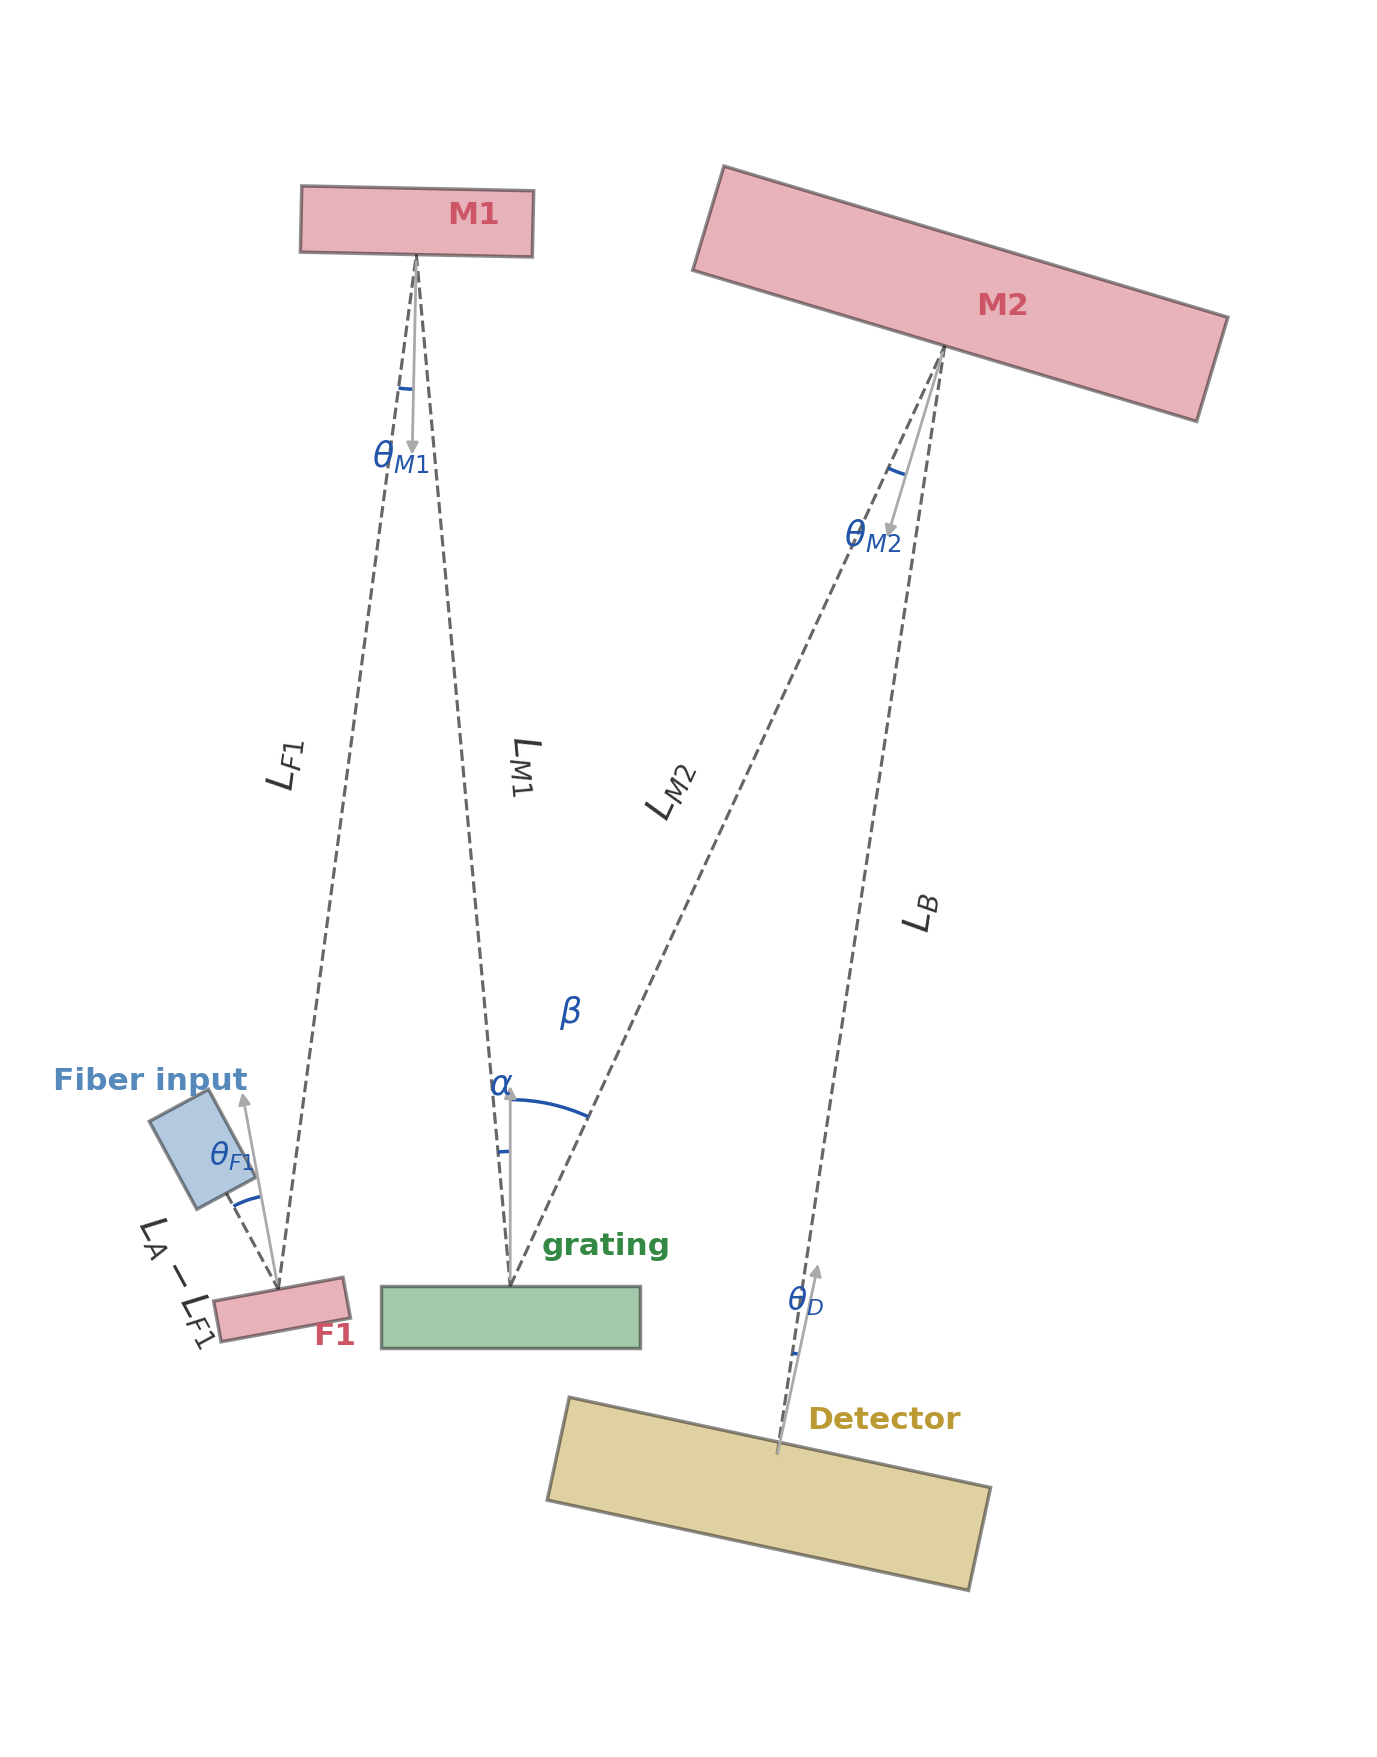
\includegraphics[width=\textwidth]{figures/fig_2_layout.png}
\caption{Top-down layout of the Czerny-Turner spectrograph showing
  the beam path from the fiber input through fold mirror F1,
  collimator M1, grating, focuser M2, and detector. Distance
  parameters ($L_{M1}$, $L_{M2}$, $L_{F1}$, $L_A$, $L_B$) label each
  arm; incidence angles ($\alpha$, $\beta$, $\theta_{M1}$,
  $\theta_{M2}$, $\theta_{F1}$, $\theta_D$) are marked at each
  surface.}
\label{fig:layout}
\end{figure}

\subsection{Czerny-Turner geometry}

The grating is fixed at the coordinate origin with its surface normal
along $+y$; all element positions are derived relative to this
reference. M1 sits in the $-x$ half-plane, M2 in the $+x$ half-plane,
and all elements lie in the $xy$ plane ($z = 0$).

The layout is described by the design parameters in
Table~\ref{tab:genome}. Mirror positions are set by ($\alpha$,
$L_{M1}$) and ($\beta$, $L_{M2}$). Slit and detector positions follow
from ($\theta_{M1}$, $L_A$) and ($\theta_{M2}$, $L_B$). When a fold
mirror is present, it is placed at distance $L_{F1}$ along the
entrance arm, deflecting the beam by $2\theta_{F1}$.

We stress that mirror incidence angles ($\theta_{M1}$, $\theta_{M2}$)
are independent of grating arm angles ($\alpha$, $\beta$). This
decoupling is essential: the Shafer condition requires
$\theta_{M1} \neq \alpha$ in general.

\begin{table}[h]
\centering
\caption{Czerny-Turner design parameters. DoFs 1--9 are always
present; DoFs 10--11 are present only when a fold mirror is active. The
deviation angle ($D_v = \alpha + \beta$) and BOM part selection are
also GA-evolved; they determine $\alpha$, $\beta$ via the grating
equation.}
\label{tab:genome}
\small
\begin{tabular*}{\textwidth}{@{\extracolsep{\fill}}clll@{}}
\toprule
DoF & Symbol & Description & Role \\
\midrule
1 & $\alpha$ & Grating incidence angle & Derived (grating eq.\ at $\lambda_c$) \\
2 & $\beta$ & Grating diffraction angle & Derived (grating eq.\ at $\lambda_c$) \\
3 & $\theta_{M1}$ & M1 incidence angle & GA-evolved \\
4 & $\theta_{M2}$ & M2 incidence angle & Derived (Shafer) \\
5 & $L_A$ & Slit to M1 distance & Derived (Coddington); NM-refined \\
6 & $L_B$ & M2 to detector distance & Derived (Coddington); NM-refined \\
7 & $L_{M1}$ & Grating to M1 distance & Grid-swept; NM-refined \\
8 & $L_{M2}$ & Grating to M2 distance & Grid-swept; NM-refined \\
9 & $\theta_D$ & Detector tilt (CW from $+z$) & NM-refined (seeded at $0^\circ$) \\
10 & $\theta_{F1}$ & F1 fold incidence angle & GA-evolved; NM-refined \\
11 & $L_{F1}$ & M1 to F1 distance & Derived (Eq.~\ref{eq:astig-free} or feasible-band midpoint) \\
\bottomrule
\end{tabular*}
\end{table}

\subsubsection{Physics-seeded optimization}
\label{sec:gauge}

The GA evolves only the deviation angle $D_v$ and $\theta_{M1}$; the
remaining parameters are derived:

\begin{itemize}[nosep]
  \item $\alpha$, $\beta$ from the grating equation at $\lambda_c$.
  \item $\theta_{M2}$ from the Shafer condition
    (Equation~\ref{eq:shafer-coma}).
  \item $L_A$, $L_B$ from the Coddington tangential focal lengths
    (Equation~\ref{eq:coddington}).
  \item $L_{F1}$ from the astigmatism-free condition
    (Equation~\ref{eq:astig-free}) for cylindrical folds, or the
    feasible-band midpoint for flat folds.
\end{itemize}

These are starting points, not final answers. The Nelder-Mead stage
perturbs $L_A$, $L_B$, $\theta_{F1}$, and $\theta_D$ away from their
seeds, allowing the optimizer to balance aberrations against detector
tilt as the ray-traced fitness dictates.

\subsection{Scene and World builder}

The geometry module produces a topology-agnostic \texttt{Scene}: an
ordered list of element placements (label, kind, position, axis, params).
The World builder translates the Scene into a raysect World (mm~$\to$~m),
realizing each element as a primitive with a custom material: spherical
and cylindrical mirrors (with optional vendor reflectance curves), a
blazed diffraction grating (vendor efficiency or analytical
$\operatorname{sinc}^2$), flat fold mirrors, and a transparent
\texttt{HitRecorder} overlay for spot-diagram capture. The entrance
aperture is a uniform-radiance emitter matching the fiber NA and core
diameter.

\subsection{Scene and CAD builder}

The same Scene that passes fitness evaluation is exported as manufactured
geometry via build123d \cite{build123d}, a Python CAD framework built on
the OpenCascade BREP kernel.  Both consumers---raysect for ray tracing,
build123d for solid modeling---read from the same BOM definitions and
Scene layout, so the manufactured geometry is guaranteed to match what
was simulated.  Housing geometry, mount footprints, beam-cone quads, wall
keep-outs, and endmill-radius fillets are all generated procedurally
from the optical layout and rebuild automatically when the optical train
changes.

The manufactured output is a single 3D-printed housing that serves as
both structural chassis and light-tight enclosure.  Optic mounts bolt to
the housing floor via screws; the HASMA fiber adapter threads into the
entrance wall via a 1/4''-36 tapped hole (tap drill printed, tapped
post-print with a conical tap guide fixture).  Each mount integrates
two-axis adjustment: pitch via a living-hinge flexure at the rear wall,
and roll via a 2-bladed leaf-spring cross-pivot section whose virtual
pivot coincides with the optic centre.  The pitch hinge foot is trimmed
at 2\textdegree{} to preload the flexure; the roll flexure is actuated
by a pair of M2 setscrews through heat-set inserts in the foot, pushing
against trapezoidal pedestals that anchor the leaf blades.  Captive TPU
contact bumps provide three-point optic retention; the top setscrew
preloads the optic against the two bottom bumps.  Three mount types
cover the optical train: mirror (round), grating (square), and OAP
(plate with hex bolt pattern).  When no vendor STEP file is registered for a given optic, the
exporter generates a procedural solid from the BOM's geometry parameters
(radius of curvature, diameter, thickness) using build123d CSG
primitives---sphere-cylinder intersections for spherical mirrors,
cylinder-cylinder for cylindrical mirrors, and so on.

The CAD builder translates each Scene element into sketch-driven
\texttt{BuildPart} constructions.  Unlike the World builder, which
converts millimeters to meters at the raysect boundary, the CAD builder
works in millimeters natively---matching the BOM and STEP conventions.
Two output formats are
produced: \textbf{STEP} (optic solids, flexure mounts, and unibody
housing assembled in their design-time poses) and \textbf{PNG}
(raysect-rendered scene visualization with physically accurate lighting).

\subsection{Forward ray tracing}

For each fitness wavelength, rays are launched from the entrance fiber
into the $f/\#$ cone and propagated through the full optical train.  A
transparent \texttt{HitRecorder} box at the detector plane captures all
intersections without attenuating the beam; mount fixtures are included
as Lambert-material CSG objects, so mount shadows are scored naturally
through reduced hit counts.  Crucially, stray light is scored rather
than filtered: all rays reaching the detector contribute to the RMS
spot, penalizing designs with poor stray-light rejection.

The forward trace yields three quantities per wavelength: (1)~RMS spot
radius (the fitness target); (2)~tangential and sagittal spot
decomposition ($\sigma_x$, $\sigma_y$, ratio, skewness); and
(3)~geometric throughput, enforced as a 0.5\% minimum constraint.
Evaluation proceeds in two tiers: an analytical pre-filter rejects
candidates where any fitness wavelength falls off the CCD (zero ray
cost), followed by the ray trace itself (1,000~rays/$\lambda$ for
coarse grid sweeps; 5,000~rays/$\lambda$ for Nelder-Mead refinement).

\subsection{Fitness function}

The scalar fitness is the mean per-wavelength RMS spot radius:
\begin{equation}
  \text{fitness} = \frac{1}{N_\lambda} \sum_\lambda
    \text{RMS}(\lambda) \quad [\mu\text{m}]
  \label{eq:fitness}
\end{equation}
Lower is better. Throughput is enforced as a 0.5\% minimum-throughput
constraint (not optimized). Infeasible candidates (optic collisions,
beam-cone clipping, mount overlaps) receive penalty fitness $10^6$
without being traced; collision detection uses the Separating Axis
Theorem on 2-D convex polygons at the optical center height.

\subsection{Evolutionary optimization}

The optimization uses the GA engine from the \texttt{evolutionary-solver}
library \cite{evosolver}, which provides the population management,
coarse grid sweep, and Nelder-Mead basin refinement stages.
The GA searches a 2D continuous space (deviation angle $D_v$,
$\theta_{M1}$) plus discrete BOM part selection. User-specified
performance targets (resolution, bandwidth, $f$-number, center
wavelength) drive BOM filtering at startup; only valid part
combinations enter the search.

\subsubsection{Evaluation flow}

\begin{enumerate}[nosep]
  \item GA proposes ($D_v$, $\theta_{M1}$, [$\theta_{F1}$], combo\_id).
  \item \texttt{expand\_genome()} derives all remaining parameters
    (Table~\ref{tab:genome}).
  \item Coarse sweep over ($L_{M1}$, $L_{M2}$): Tier~1 pre-filter
    then Tier~2 forward trace at 1k rays/$\lambda$.
  \item Basin extraction; Nelder-Mead refines ($L_{M1}$, $L_{M2}$,
    $L_A$, $\theta_{F1}$, $L_B$, $\theta_D$) at 5k rays/$\lambda$.
  \item Best basin fitness $\to$ candidate score.
\end{enumerate}

The GA defaults to point-source evaluation (\texttt{-{}-point\_source}).
When the extended source is used instead, the 25\,$\mu$m fiber
convolution dominates the tangential spot width, masking the
aberration differences between candidates; the optimizer loses
sensitivity to optical quality and converges on layouts that minimize
sagittal extent rather than tangential resolution. Point-source
evaluation isolates the aberration structure, allowing the GA to
select for the optical merit that matters once the slit image is
convolved in post.

\subsection{Validation}

We validated the simulation pipeline against Xia \textit{et al.}\
\cite{xia2017}, who published Zemax-computed RMS spot diagrams for both
a standard and an aberration-corrected Czerny-Turner spectrometer
(350--750\,nm, 600\,g/mm, 25\,$\mu$m slit, $f/5$). All validation results
were obtained with a point source (no fiber convolution), matching
Xia's Zemax configuration. The validation has three parts:
(a)~forward-trace reproduction of their standard Czerny-Turner geometry,
(b)~Nelder-Mead refinement of their aberration-corrected Czerny-Turner, and
(c)~independent GA convergence to the same performance class.

\subsubsection{Standard Czerny-Turner: forward-trace match}
\label{sec:standard-ct}

Xia's standard Czerny-Turner ($R_{M1} = 224$\,mm, $R_{M2} = 220$\,mm,
$\theta_D = 3.5^\circ$) is encoded as a BOM
(\texttt{czerny\_bom\_xia2017\_standard.toml}) and baseline layout
(\texttt{czerny\_baseline\_xia2017.toml}). Sections~3.9.1 and 3.9.2
are produced by a single script:

\begin{quote}
\small\ttfamily
python scripts/validate\_xia2017.py
\end{quote}

\noindent Our forward-trace results were:

\begin{center}
\begin{tabular}{@{}cccc@{}}
\toprule
$\lambda$ (nm) & Our RMS ($\mu$m) & Xia Fig~5a ($\mu$m) & Difference \\
\midrule
350 & 105.7 & 101.5 & $+4\%$ \\
450 & 132.8 & 132.6 & $+0.1\%$ \\
550 & 179.2 & 180.8 & $-1\%$ \\
650 & 246.1 & 248.9 & $-1\%$ \\
750 & 335.8 & 336.8 & $-0.3\%$ \\
\midrule
\textbf{mean} & \textbf{199.9} & \textbf{200.1} & $\mathbf{-0.1\%}$ \\
\bottomrule
\end{tabular}
\end{center}

All five wavelengths agreed within 5\%, confirming that our
forward-trace simulation reproduces Zemax results when given identical
geometry.

\subsubsection{Aberration-corrected Czerny-Turner: Nelder-Mead refinement}

Xia's aberration-corrected Czerny-Turner replaces the flat fold with a sagittal
cylindrical mirror ($R_{F1} = 20$\,mm) and converts the collimator to
tangential cylindrical ($R_{M1} = 224$\,mm). This BOM is encoded in
\texttt{czerny\_bom\_xia2017\_corrected.toml}. The following parameters were held
fixed (constrained by Xia's geometry):

\begin{center}
\begin{tabular}{@{}lc@{}}
\toprule
Parameter & Value \\
\midrule
$\alpha$ & $5.16^\circ$ \\
$\beta$ & $-24.84^\circ$ \\
$\theta_{M1}$ & $6.4^\circ$ \\
$\theta_{M2}$ & $8.1^\circ$ \\
$\theta_{F1}$ & $18.0^\circ$ \\
$L_A$ & 111.30\,mm \\
\bottomrule
\end{tabular}
\end{center}

At Xia's reported layout values, our simulations showed RMS spot size
asymmetry at the edge wavelengths, suggesting the presence of residual
aberrations. We ran a Nelder-Mead optimization over the
remaining free parameters ($L_{F1}$, $L_B$, $\theta_D$):

\begin{center}
\begin{tabular}{@{}lclcc@{}}
\toprule
Parameter & Value & Xia notation & Xia Table~2 & Shift \\
\midrule
$L_A - L_{F1}$ & 10.531\,mm & $l_{SM1}$ & 10.526\,mm & $+0.005$\,mm \\
$L_{F1}$ & 100.771\,mm & $l_{M1M2}$ & 100.774\,mm & $-0.003$\,mm \\
$L_B$ & 108.872\,mm & $l_{M3D}$ & 108.751\,mm & $+0.121$\,mm \\
$\theta_D$ & $4.30^\circ$ & $\theta_D$ & $3.50^\circ$ & $+0.80^\circ$ \\
\bottomrule
\end{tabular}
\end{center}

The fold distance shifted by only 0.005\,mm, confirming that the
astigmatism-free condition tightly constrains the fold placement. The
per-wavelength RMS spots before and after optimization were:

\begin{center}
\begin{tabular}{@{}ccccc@{}}
\toprule
$\lambda$ (nm) & Before optimization ($\mu$m) & After optimization ($\mu$m) & Xia Fig~5b ($\mu$m) & Difference \\
\midrule
350 & 12.2 & 15.3 & 16.7 & $-9\%$ \\
450 & 6.5 & 8.1 & 8.2 & $-1\%$ \\
550 & 4.5 & 7.2 & 4.4 & $+63\%$ \\
650 & 11.9 & 7.3 & 9.0 & $-19\%$ \\
750 & 28.5 & 15.6 & 16.9 & $-8\%$ \\
\midrule
\textbf{mean} & \textbf{12.7} & \textbf{10.7} & \textbf{11.0} & $\mathbf{-3\%}$ \\
\bottomrule
\end{tabular}
\end{center}

After optimization the mean RMS agreed with Xia's result within 3\%
and the band-edge asymmetry collapsed (750\,nm: 28.5 $\to$
15.6\,$\mu$m), but at the cost of the center wavelength: 550\,nm
degraded from 4.5 to 7.2\,$\mu$m ($+63\%$ above Xia's 4.4\,$\mu$m).
The source of the per-wavelength discrepancies remains unresolved.

\subsubsection{Aberration-corrected Czerny-Turner: GA convergence}

As a final validation, we ran the full GA pipeline against Xia's
aberration-corrected Czerny-Turner BOM without constraining the
deviation angle or mirror incidence angles:

\begin{quote}
\small\ttfamily
python run\_optimizer.py czerny -{}-bom data/czerny\_bom\_xia2017\_corrected.toml \textbackslash\\
\hspace*{2em} -{}-max\_rld 17 -{}-min\_bw 400 -{}-max\_fnum 5 -{}-center 550 \textbackslash\\
\hspace*{2em} -{}-fold\_mode F1 -{}-pop\_size 128
\end{quote}

\noindent The run converged in 11~generations (128~candidates each,
point source, 350--750\,nm bandwidth).  The GA independently
discovered a different angular configuration, exported as
\texttt{czerny\_baseline\_xia2017\_evolved.toml}:

\begin{center}
\begin{tabular}{@{}lcc@{}}
\toprule
Parameter & Xia Fig~5b & GA winner \\
\midrule
$\alpha$ & 5.2\textdegree & 3.20\textdegree \\
$\beta$ & $-$24.8\textdegree & $-$22.70\textdegree \\
$\theta_{M1}$ & 6.4\textdegree & 10.2\textdegree \\
$\theta_{M2}$ & 8.1\textdegree & 12.2\textdegree \\
$\theta_{F1}$ & 18.0\textdegree & 34.0\textdegree \\
$\theta_D$ & 3.50\textdegree & 4.92\textdegree \\
$L_A$ & 111.30\,mm & 104.27\,mm \\
$L_{F1}$ & 100.77\,mm & 92.22\,mm \\
$L_A - L_{F1}$ & 10.53\,mm & 12.04\,mm \\
$L_B$ & 108.75\,mm & 114.17\,mm \\
$L_{M1}$ & --- & 91.53\,mm \\
$L_{M2}$ & --- & 86.74\,mm \\
\bottomrule
\end{tabular}
\end{center}

The per-wavelength RMS spots at the three fitness wavelengths were:

\begin{center}
\begin{tabular}{@{}cccc@{}}
\toprule
$\lambda$ & Xia Fig~5b & GA winner & Difference \\
\midrule
350\,nm & 16.7\,$\mu$m & 18.7\,$\mu$m & $+12\%$ \\
550\,nm & 4.4\,$\mu$m & 6.3\,$\mu$m & $+43\%$ \\
750\,nm & 16.9\,$\mu$m & 24.1\,$\mu$m & $+43\%$ \\
\midrule
\textbf{mean} & \textbf{12.7}\,$\mu$m & \textbf{16.4}\,$\mu$m & $\mathbf{+29\%}$ \\
\bottomrule
\end{tabular}
\end{center}

Crucially, the GA was subject to a packaging constraint absent from
Xia's Zemax model: the TCD1304 PCBA (70$\times$40\,mm) collides with
the grating mount at Xia's arm lengths.  To resolve this collision,
the GA steepened the mirror incidence angles
($\theta_{M1}$: $6.4^\circ \to 10.2^\circ$; $\theta_{M2}$:
$8.1^\circ \to 12.2^\circ$), thereby splaying the beam path to
clear the board.  However, steeper mirrors necessarily increase
off-axis astigmatism ($\Delta f \propto \sin^2\theta / \cos\theta$),
and consequently the fold must compensate: $\theta_{F1}$ steepens
from $18^\circ$ to $34^\circ$, with $L_{F1}$ following from
Equation~\ref{eq:astig-free}.  Nonetheless, the resulting mean RMS
(16.4\,$\mu$m vs Xia's 12.7\,$\mu$m) remains an order of magnitude
better than the 200\,$\mu$m standard Czerny-Turner
(Section~\ref{sec:standard-ct}), confirming that the GA converges
to the correct performance class while respecting physical packaging
constraints that a pure optical optimization would not encounter.

As a demonstration of the capabilities of the ray tracing pipeline,
Figure~\ref{fig:beam-profile} shows the beam footprint at 550\,nm
through the GA winner's optical train, generated with:

\begin{quote}
\small\ttfamily
python scripts/beam\_profile.py \textbackslash\\
\hspace*{2em} -{}-baseline data/czerny\_baseline\_xia2017\_evolved.toml \textbackslash\\
\hspace*{2em} -{}-bom data/czerny\_bom\_xia2017\_corrected.toml -{}-point\_source -{}-no-title
\end{quote}

\begin{figure}[ht!]
\centering
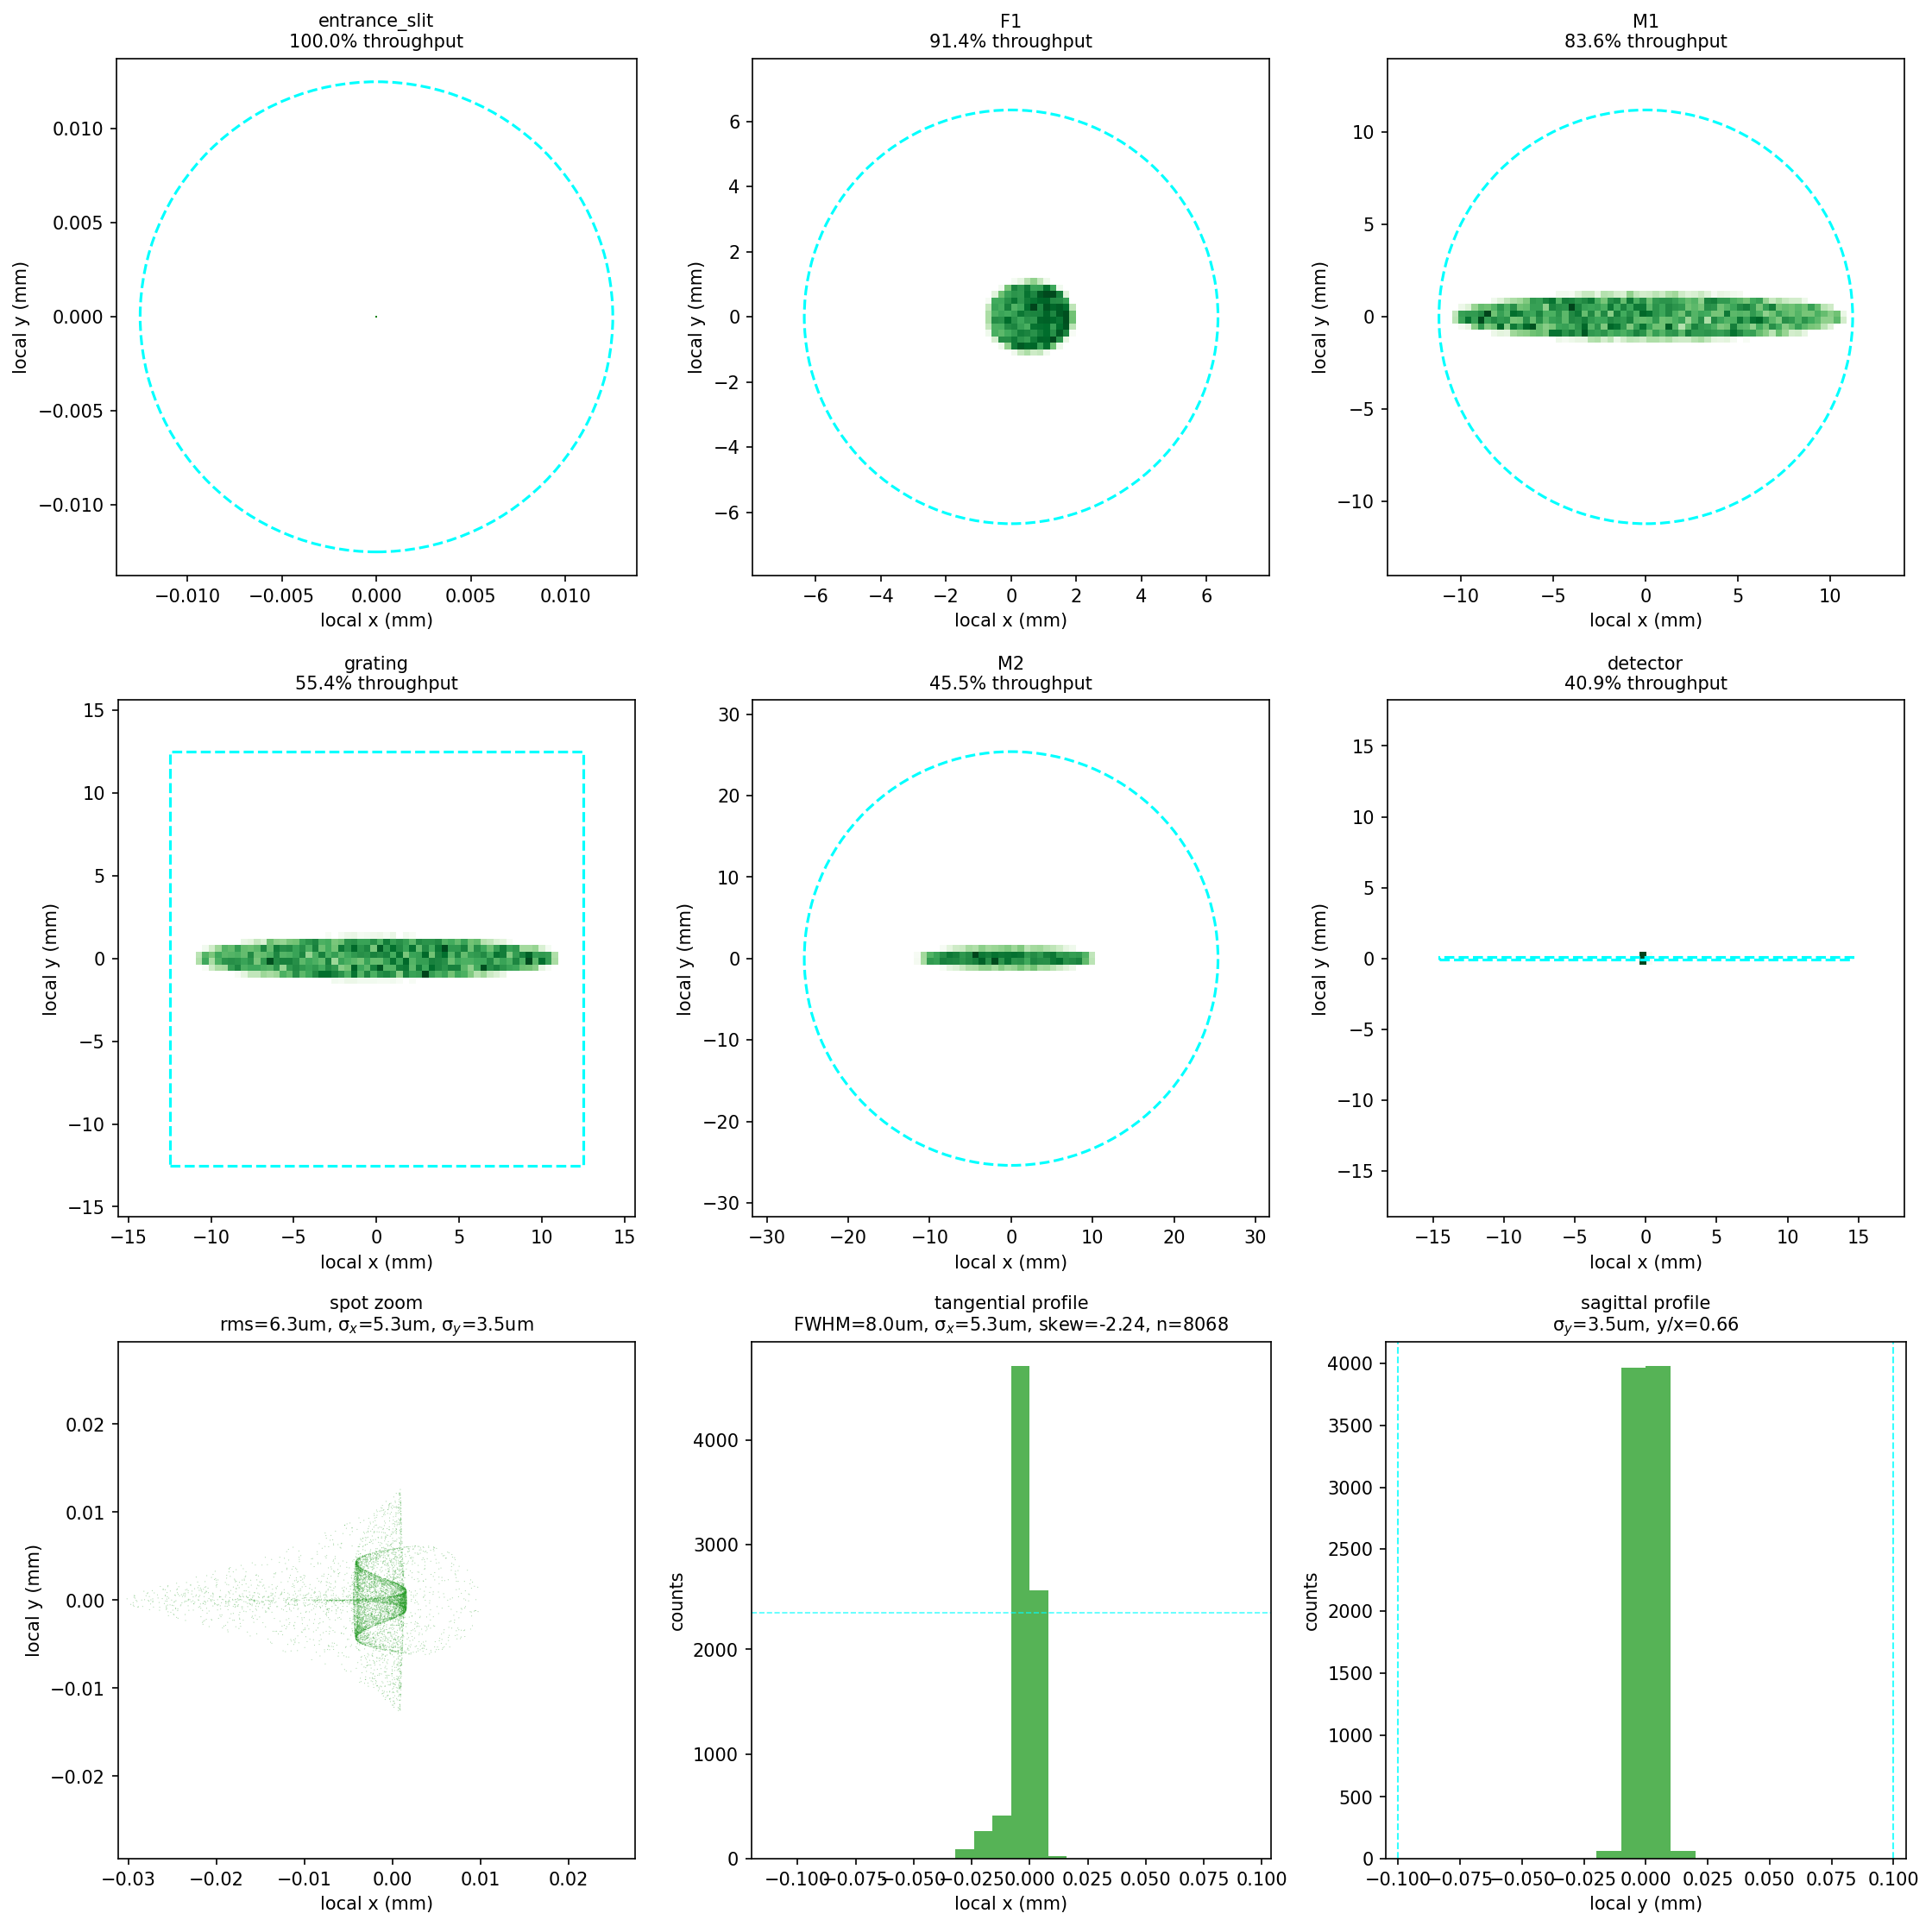
\includegraphics[width=\textwidth]{figures/fig_3_beam_profile.png}
\caption{Beam footprint at 550\,nm through the GA-evolved
aberration-corrected Czerny-Turner (point source, 10\,000 rays).
Top two rows: beam on each surface with aperture boundary (cyan) and
cumulative
throughput. Bottom row: spot diagram with RMS decomposition
($\sigma_x = 5.2$\,$\mu$m, $\sigma_y = 3.5$\,$\mu$m), tangential
profile with FWHM, and sagittal profile.}
\label{fig:beam-profile}
\end{figure}

\clearpage
%% ===================================================================
\section{Instrument Control Software}
\label{sec:software}
%% ===================================================================

\textit{We describe \texttt{controller}, our client for the TCD1304
detector: a desktop application for live viewing, capture, and
wavelength calibration, with a command-line layer for scripting and
offline reprocessing.  The instrument requires drmcnelson's open
firmware \cite{tcd1304board} on its Teensy controller board; beyond
that, \texttt{controller} handles everything on the host.}

\subsection{Architecture}

Running \texttt{controller} with no arguments launches the desktop
application, the primary tool.  Subcommands expose the same
underlying library for scripting and for reprocessing saved captures,
and the library itself is importable for custom analysis.  A single
worker thread owns the serial port, so only one client can talk to
the instrument at a time.

\subsection{Acquisition}
\label{sec:acquisition}

The firmware operates the sensor in two timing modes
\cite{tcd1304board}.  In periodic interrupt timer (PIT) or ``single
pulse'' mode, the exposure time sets the frame interval and frames
arrive back to back; exposure has no practical upper limit.
In pulse-loop mode (PLM), the firmware collects fast frame sets with
exposures down to microseconds and clears residual charge internally
between frames; the frame interval must cover the readout plus the
exposure.
\texttt{controller} selects the mode automatically
(Table~\ref{tab:acq-modes}).

\begin{table}[ht]
\centering
\caption{Acquisition modes.}
\label{tab:acq-modes}
\small
\begin{tabular}{@{}lll@{}}
\toprule
Mode & Exposure & Character \\
\midrule
PIT + clearing & $\geq 16$\,ms & ghost-free; the default for
quantitative work \\
PLM & 1--15\,ms & bright-line regime only (see text) \\
\bottomrule
\end{tabular}
\end{table}

\texttt{controller} handles the firmware's quirks automatically: it
runs the clearing engine in PIT mode (frames otherwise carry a
residual ghost charge), pads PLM frame intervals to crash-safe
values, discards the contaminated leading frames of every read, and
sets the recommended sensor clock on every connect.  One caveat: PLM
sacrifices photometric fidelity at short exposures (weak signals read
low and backgrounds are not flat), so we suggest using it as a
bright-line mode and recommend doing quantitative work in PIT.

\subsection{Calibration}
\label{sec:calibration}

We calibrate against six index lines of an ordinary compact
fluorescent lamp (Table~\ref{tab:cfl-lines}), listed in
\texttt{data/cfl\_lines.toml} as reference wavelengths plus the
nominal dispersion.

\begin{table}[ht]
\centering
\caption{CFL wavelength calibration index lines.}
\label{tab:cfl-lines}
\small
\begin{tabular*}{0.85\textwidth}{@{\extracolsep{\fill}}lll@{}}
\toprule
Wavelength (nm) & Species & Fit \\
\midrule
404.656 & Hg & single Gaussian \\
435.833 & Hg & single Gaussian \\
542.4   & Tb$^{3+}$ & joint two-Gaussian (blend) \\
546.074 & Hg & joint two-Gaussian (blend) \\
611.6   & Eu$^{3+}$ & core-weighted, fixed baseline \\
631.3   & Eu$^{3+}$ & single Gaussian \\
\bottomrule
\end{tabular*}
\end{table}

A pattern locator finds the six lines from scratch on each run (any
shift, $\pm 25$\% of nominal dispersion), saturation-masked Gaussian
fits refine each peak center, and a quadratic fit to the six centers
yields the wavelength solution $\lambda(p) = a_0 + a_1 p + a_2 p^2$.

\subsection{Interfaces}

\subsubsection{Desktop application}

The desktop application presents one window
(Figure~\ref{fig:controller-gui}, controls in
Table~\ref{tab:gui-controls}): a set of controls along the top row
drives live spectral acquisition, and \ui{Capture to file} saves the
current acquisition.
Captures use the \texttt{.tcd1304} plain-text format
\cite{tcd1304board}; \texttt{controller} extends the header with the
firmware identifier, stored wavelength coefficients, acquisition
mode, clearing pulse count, and exposure, so anyone can audit the
photometric regime of a file after the fact.

Clicking \ui{Calibrate\ldots} opens the live calibration panel, where every frame receives the line location
and fit of Section~\ref{sec:calibration} and the fitted coefficients
update on screen.  \ui{Store to device} writes the latest fit and
verifies it by readback; \ui{Cancel} or \ui{$\times$} closes the
panel without saving.

If the USB connection drops, the application retries automatically;
if the retries fail, pressing the \ui{Reconnect} button beside the
device indicator re-establishes the connection.

\begin{figure}[ht]
\centering
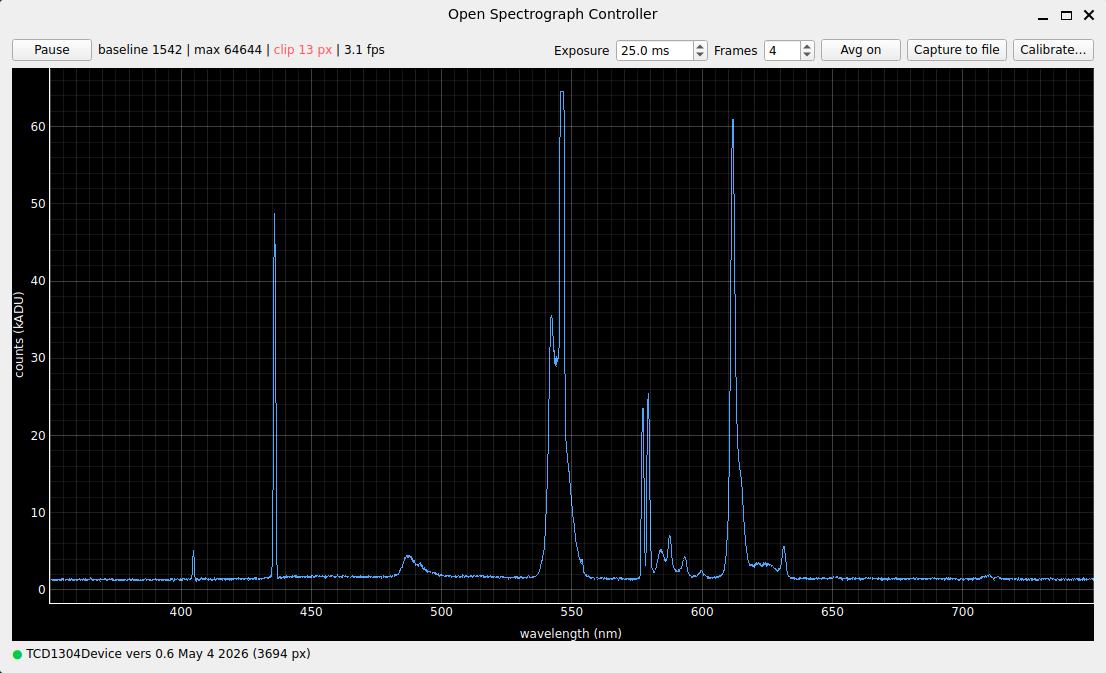
\includegraphics[width=\textwidth]{figures/fig_4_controller_gui.png}
\caption{The \texttt{controller} desktop application showing a live
CFL spectrum (25\,ms exposure, PIT mode).}
\label{fig:controller-gui}
\end{figure}

\begin{table}[ht]
\centering
\caption{Desktop application controls.}
\label{tab:gui-controls}
\small
\begin{tabular}{@{}lp{11cm}@{}}
\toprule
Control & Function \\
\midrule
\ui{Pause} / \ui{Resume} & freeze or resume the live view \\
Metrics readout & per-frame baseline, clipped pixels, maximum,
display rate \\
\ui{Exposure} & exposure time; automatically selects the
acquisition mode (PIT or PLM) \\
\ui{Frames} & frames per capture, and per averaged update when
averaging is on \\
\ui{Avg on} / \ui{Avg off} & toggle averaging of the live view
over the frame count \\
\ui{Capture to file} & write the current acquisition to a
\texttt{.tcd1304} file in \texttt{output/} \\
\ui{Calibrate\ldots} & open the live calibration panel \\
Status bar & shows connection indicator, firmware identity, status
messages \\
\bottomrule
\end{tabular}
\end{table}

\subsubsection{Command-line interface}

\texttt{controller} also exposes a command-line interface with
subcommands to support scripting and offline work
(Table~\ref{tab:controller-cli}).

\begin{table}[ht]
\centering
\caption{\texttt{controller} command-line interface.}
\label{tab:controller-cli}
\small
\begin{tabular}{@{}ll@{}}
\toprule
Command & Function \\
\midrule
\texttt{controller capture} & acquire clean frames to a
\texttt{.tcd1304} file \\
\texttt{controller calibrate} & fit lines and constants (saved file
or \texttt{-{}-live}) \\
\texttt{controller plot} & plot a capture on its recorded wavelength
axis \\
\texttt{controller info} & report firmware version, configuration,
coefficients, temperature \\
\texttt{controller ports} & list the serial devices the host can
see \\
\texttt{controller store} / \texttt{erase} & manage on-device
coefficients \\
\bottomrule
\end{tabular}
\end{table}

\clearpage
%% ===================================================================
\section{The v0 Design}
\label{sec:v0-design}
%% ===================================================================

\textit{We present a catalog-parts build that validates the simulation
pipeline end-to-end and provides the fastest path to a physical
prototype.}

\begin{figure}[htbp]
\centering
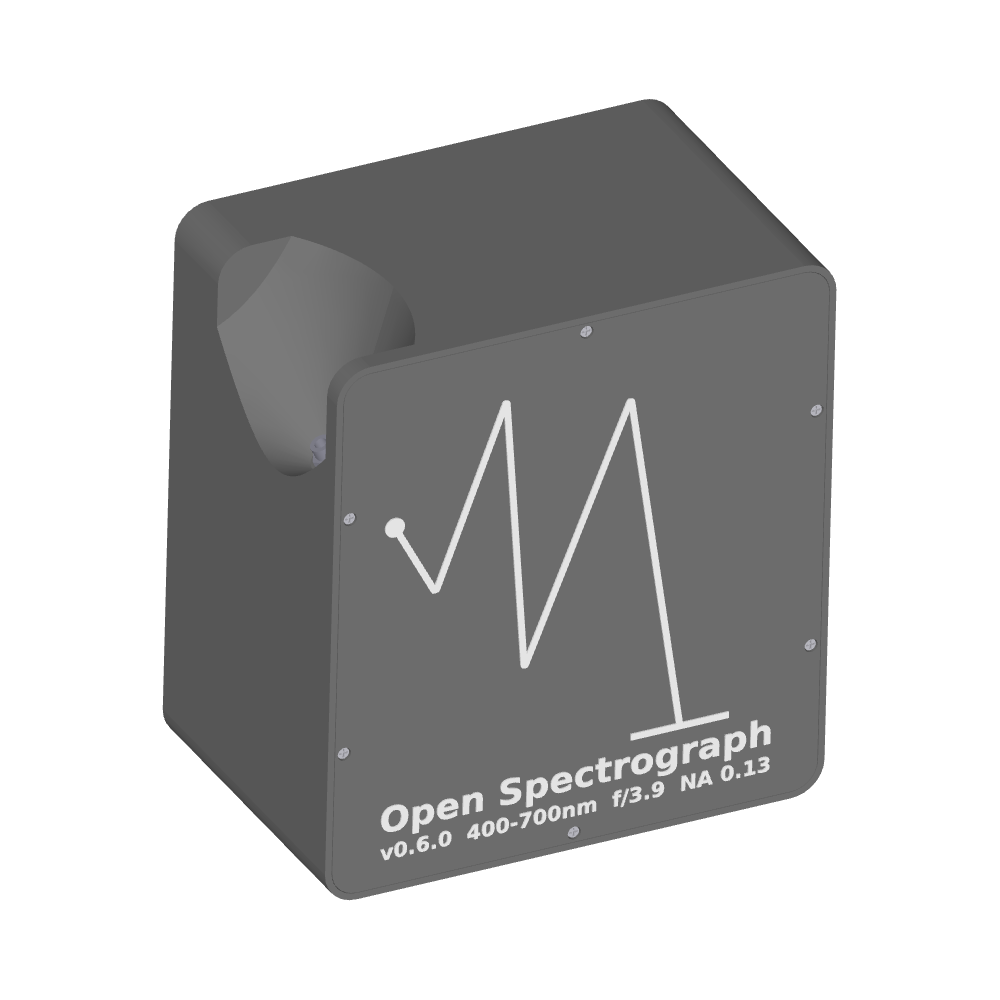
\includegraphics[width=\linewidth]{figures/fig_5_v0-model.png}
\caption{CAD model of the v0.6.0 assembly.}
\label{fig:v0-model}
\end{figure}

\subsection{Optical train}

The v0 optical train is an aberration-corrected Czerny-Turner with a
tangential cylindrical collimator (M1), sagittal cylindrical
collimator (F1), and spherical focuser (M2):

\begin{center}
\begin{tabular}{@{}lllr@{}}
\toprule
Element & Specification & Part & Cost \\
\midrule
Fiber & 25\,$\mu$m core, NA~0.12 & SMA-905 & --- \\
Adapter & SMA bulkhead, 1/4''-36 thread & HASMA & \$10 \\
F1 & $f = 25$\,mm, $\varnothing\,25.4$\,mm, cyl.\ sagittal & CCM254-025-G01 & \$201 \\
M1 & $f = 100$\,mm, $\varnothing\,25.4$\,mm, cyl.\ tangential & CCM254-100-G01 & \$201 \\
Grating & 600\,g/mm, 25$\times$25\,mm, blaze 500\,nm & GR25-0605 & \$137 \\
M2 & $f = 100$\,mm, $\varnothing\,50.8$\,mm, spherical & CM508-100-G01 & \$138 \\
Detector board & 3648\,px, 8\,$\mu$m pitch, 16-bit ADC & TCD1304 SPI Rev2EB & \$110 \\
Controller board & Teensy~4.0, FlexPWM, USB~2.0 HS & Instr.\ Controller & \$90 \\
Hardware & inserts, setscrews, screws & McMaster-Carr & \$12 \\
Housing & 3D printed black plastic & 5 parts + 4 mounts & \$5 \\
\midrule
& & \textbf{Total} & \textbf{\$904} \\
\bottomrule
\end{tabular}
\end{center}

All optics are Thorlabs catalog parts; the GA was run with:

\begin{quote}
\small\ttfamily
python run\_optimizer.py czerny -{}-bom data/czerny\_bom\_v0\_design.toml \textbackslash\\
\hspace*{2em} -{}-max\_rld 17 -{}-min\_bw 300 -{}-max\_fnum 4 -{}-center 550 \textbackslash\\
\hspace*{2em} -{}-fold\_mode F1 -{}-pop\_size 128
\end{quote}

The GA optimizer (point source, 128 population, 7 generations)
converged to the following layout, exported as
\texttt{czerny\_baseline\_v0\_design.toml}:

\begin{center}
\begin{tabular}{@{}lr@{}}
\toprule
Parameter & Value \\
\midrule
$\alpha$        & 3.49\textdegree \\
$\beta$         & $-$23.01\textdegree \\
$\theta_{M1}$   & 12.5\textdegree \\
$\theta_{M2}$   & 15.41\textdegree \\
$\theta_{F1}$   & 24.4\textdegree \\
$\theta_D$      & 9.2\textdegree \\
$L_A$           & 86.6\,mm \\
$L_{F1}$        & 59.5\,mm \\
$L_A - L_{F1}$  & 27.1\,mm \\
$L_B$           & 109.3\,mm \\
$L_{M1}$        & 86.9\,mm \\
$L_{M2}$        & 83.8\,mm \\
\bottomrule
\end{tabular}
\end{center}

Thorlabs is the only Western manufacturer stocking concave cylindrical
mirrors, and the shortest available focal length is $f = 25$\,mm
(CCM254-025-G01).  This is twice the ideal F1 focal length for this
geometry, forcing the optimizer into steeper incidence angles and a
wider layout with higher residual aberrations at the band edges.

\subsection{Performance}

\begin{figure}[ht!]
\centering
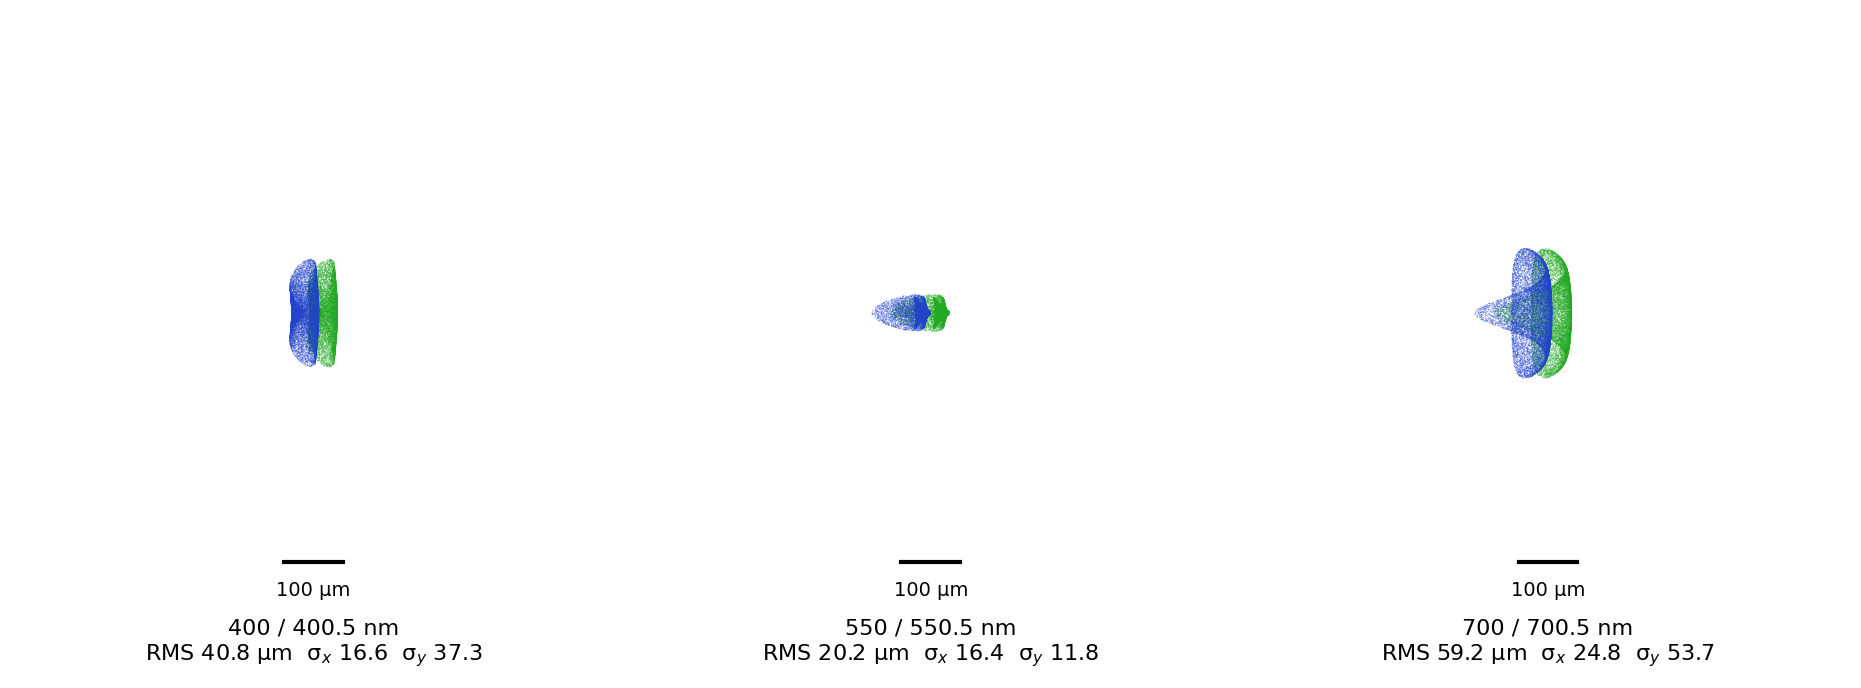
\includegraphics[width=\textwidth]{figures/fig_6a_v0_spot_pt.png}\\[0.5em]
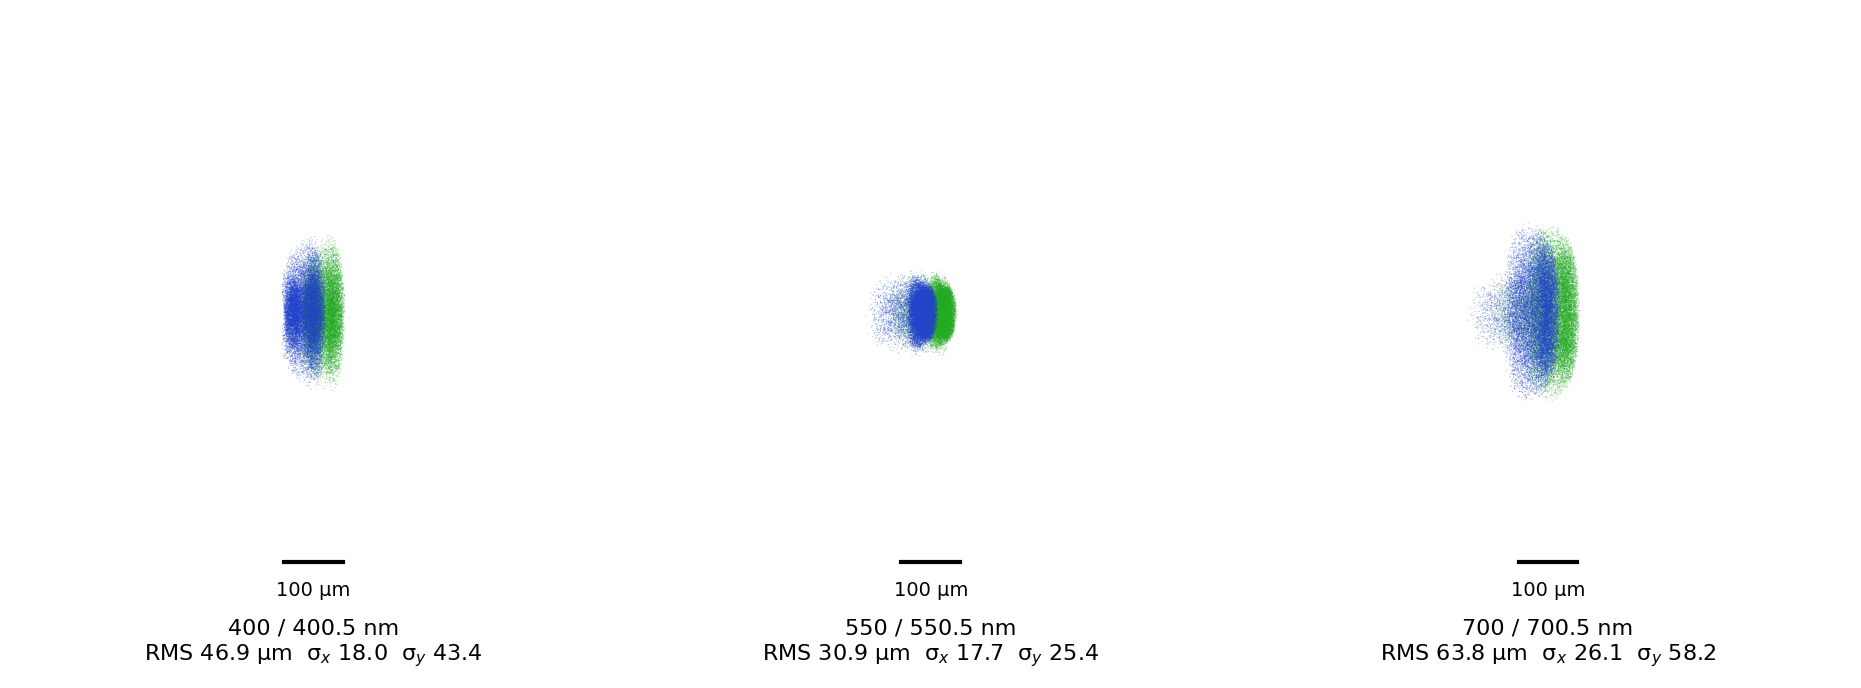
\includegraphics[width=\textwidth]{figures/fig_6b_v0_spot_ext.png}
\caption{v0 spot diagrams at 400, 550, and 700\,nm.  Each panel shows a
wavelength pair separated by $\Delta\lambda = 0.5$\,nm (green and
blue).  Top: point source (optical aberrations only).  Bottom:
25\,$\mu$m fiber source (slit-limited).  The pairs are resolved at all
three wavelengths in both cases, confirming sub-1\,nm ILF
across the band.  RMS annotation refers to the primary wavelength only.}
\label{fig:v0-spot-panel}
\end{figure}

\begin{table}[ht!]
\centering
\caption{v0 spot size and ILF performance at three wavelengths.}
\label{tab:v0-performance}
\begin{tabular}{@{}lrrrr@{}}
\toprule
& \multicolumn{2}{c}{Point source} & \multicolumn{2}{c}{25\,$\mu$m fiber} \\
\cmidrule(lr){2-3}\cmidrule(lr){4-5}
$\lambda$ (nm) & RMS ($\mu$m) & ILF EE76 (nm) & RMS ($\mu$m) & ILF EE76 (nm) \\
\midrule
400 & 41.1 & 0.68 & 46.8 & 0.74 \\
550 & 20.1 & 0.36 & 30.9 & 0.51 \\
700 & 58.5 & 0.73 & 63.3 & 0.85 \\
\midrule
Mean & 39.9 & 0.59 & 47.0 & 0.70 \\
\bottomrule
\end{tabular}
\end{table}

\noindent Figure~\ref{fig:v0-spot-panel} shows the v0 spot diagrams:
point source (top) and 25\,$\mu$m fiber source (bottom).  Both were
generated from the exported baseline:

\begin{quote}
\small\ttfamily
python scripts/spot\_panel.py \textbackslash\\
\hspace*{2em} -{}-baseline data/czerny\_baseline\_v0\_design.toml \textbackslash\\
\hspace*{2em} -{}-bom data/czerny\_bom\_v0\_design.toml -{}-no-title\\[0.5em]
python scripts/spot\_panel.py \textbackslash\\
\hspace*{2em} -{}-baseline data/czerny\_baseline\_v0\_design.toml \textbackslash\\
\hspace*{2em} -{}-bom data/czerny\_bom\_v0\_design.toml -{}-no-point\_source -{}-no-title
\end{quote}

\subsection{Assembly tolerance budget}

A true one-at-a-time (OAT) sweep perturbs each physical dimension
independently --- angular tilts $\pm 2$\textdegree, layout distances
$\pm 5\%$ --- without recomputing downstream positions, and records
the ILF (encircled-energy width containing 76\% of hits, equivalent
to Gaussian FWHM) at each point.  For each axis the table reports the
maximum perturbation that keeps the ILF below 1\,nm:

\medskip
\hspace{2em}\texttt{python scripts/tolerance.py {-}{-}rays 100000 {-}{-}n\_points 11 {-}{-}ilf\_target 1.0}
\medskip

\begin{table}[ht]
\centering
\caption{v0 assembly tolerance budget (ILF $< 1$\,nm).}
\label{tab:v0-tolerance}
\small
\begin{tabular}{rclrrl}
\toprule
Rank & Symbol & Description & Nominal & Budget & Category \\
\midrule
 1 & $L_{F1}$         & M1 to F1 distance             & 59.5\,mm        & $\pm$0.12\,mm        & tight \\
 2 & $L_A$            & Slit to M1 distance           & 86.6\,mm        & $\pm$0.21\,mm        & tight \\
 3 & $L_{M1}$         & Grating to M1 distance        & 86.9\,mm        & $\pm$0.22\,mm        & tight \\
 4 & $L_B$            & M2 to detector distance       & 109.3\,mm       & $\pm$0.24\,mm        & tight \\
 5 & $L_{M2}$         & Grating to M2 distance        & 83.8\,mm        & $\pm$0.27\,mm        & tight \\
 6 & $\theta_{M2}$    & M2 incidence angle            & 15.4\textdegree & $\pm$0.28\textdegree & tight \\
 7 & $\theta_{M1}$    & M1 incidence angle            & 12.5\textdegree & $\pm$0.41\textdegree & moderate \\
 8 & $\varphi_{F1}$   & F1 cylinder axis orientation  & 90\textdegree   & $\pm$0.48\textdegree & moderate \\
 9 & $\varphi_{M1}$   & M1 cylinder axis orientation  & 0\textdegree    & $\pm$0.57\textdegree & moderate \\
10 & $\alpha$          & Grating incidence angle       & 3.5\textdegree  & $\pm$1.94\textdegree & relaxed \\
11 & $\theta_{F1}$    & F1 fold incidence angle       & 24.4\textdegree & $>\pm$2\textdegree   & relaxed \\
12 & $\theta_D$       & Detector tilt                 & 9.2\textdegree  & $>\pm$1\textdegree   & relaxed \\
\bottomrule
\end{tabular}
\end{table}

Layout distances (ranks~1--5) have the tightest budgets: $L_{F1}$
must be held to $\pm 0.12$\,mm, and all arm lengths to
$\sim \pm 0.25$\,mm.  The M2 incidence angle $\theta_{M2}$ is
comparably tight at $\pm 0.28$\textdegree.  The cylinder axis
orientations $\varphi_{M1}$ and $\varphi_{F1}$ (ranks~8--9)
tolerate $\sim \pm 0.5$\textdegree\ deviation.  The grating
incidence angle~$\alpha$, fold angle~$\theta_{F1}$, and detector
tilt~$\theta_D$ are relaxed and do not require special attention
during assembly.

\subsection{Printable parts}

All printable parts are generated procedurally from BOM parameters
and exported with:

\medskip
\hspace{2em}\texttt{python export.py {-}{-}baseline data/czerny\_baseline\_v0\_design.toml {-}{-}cad}
\medskip

\noindent All parts were printed using a multimaterial fused deposition
modelling (FDM) printer with a 0.4\,mm nozzle at 0.24\,mm layer thickness
with 15\% gyroid infill.  Optic mounts were printed on their backs (foot
pointing up).  Supports were enabled for the alignment screen, housing, and
bottom cover; a PLA support interface was used for PETG parts for ease of
support removal.

\subsubsection{Housing and mounts}

\begin{table}[h!]
\centering
\caption{Printable housing and mount parts.}
\label{tab:printable-parts}
\small
\begin{tabular*}{\textwidth}{@{\extracolsep{\fill}}llll@{}}
\toprule
Part & File & Material & Notes \\
\midrule
Housing & \texttt{housing.step} & PETG & Unibody chassis + light-tight enclosure \\
Top cover & \texttt{top\_cover.step} & PETG & Snap-fit lid with embossed ray path \\
Detector cover & \texttt{detector\_cover.step} & PETG & Shields detector pocket \\
Bottom cover & \texttt{bottom\_cover.step} & PETG & Base plate with screw holes \\
F1 mount & \texttt{f1\_mount.step} & PETG & Sagittal cylindrical collimator mount \\
M1 mount & \texttt{m1\_mount.step} & PETG & Tangential cylindrical collimator mount \\
M2 mount & \texttt{m2\_mount.step} & PETG & Spherical focuser mount \\
Grating mount & \texttt{grating\_mount.step} & PETG & Ruled grating mount \\
Contact bumps & (in mounts) & TPU & Captive cylinders, three per mount \\
\bottomrule
\end{tabular*}
\end{table}

Each mount slots into locating ridges on the housing cavity floor, and
includes captive TPU contact bumps (three per mount) for
setscrew-preloaded three-point retention.  The HASMA bore prints as a
5.5\,mm tap drill hole; the 1/4''-36 thread is tapped post-print.

\subsubsection{Assembly fixtures}

\begin{table}[h!]
\centering
\caption{Assembly fixtures.}
\label{tab:fixtures}
\small
\begin{tabular*}{\textwidth}{@{\extracolsep{\fill}}llll@{}}
\toprule
Fixture & File & Material & Purpose \\
\midrule
M1 fixture & \texttt{m1\_fixture.step} & PETG & Holds mirror during assembly \\
M2 fixture & \texttt{m2\_fixture.step} & PETG & Holds mirror during assembly \\
F1 fixture & \texttt{f1\_fixture.step} & PETG & Holds mirror during assembly \\
Grating fixture & \texttt{grating\_fixture.step} & PETG & Holds grating during assembly \\
HASMA tap guide & \texttt{hasma\_tap\_fixture.step} & PETG & Guides 1/4''-36 tap through bore \\
Alignment screen & \texttt{alignment\_screen.step} & PETG & Beam centering target \\
\bottomrule
\end{tabular*}
\end{table}

Each fixture envelopes the mount and optic with a 1\,mm contact lip,
through-cuts beneath the foot tongue and pusher shelf to prevent
bottoming out, and a setscrew access hole.  The HASMA tap guide is a
20\,mm cone matching the housing flare, with a 1/4'' through bore for
tap alignment.  The laser alignment screen is a three-body multi-color
print (frame, white disk, black reticle) that straddles the mount foot
tongue and sits at the optic vertex plane, providing a centering target
for aligning each optic before the housing is sealed.

\subsection{Assembly procedure}

\subsubsection{Prepare housing}
Use the HASMA tap fixture to guide a 1/4''-36 tap during the tapping
process.  Slowly rotate the tap in the bore until the thread is
completely cut through the housing sidewall.  The tap must be held
perpendicular to the bore hole during this process; any misalignment
causes gross tilting and translation of the input beam.  Thread the
HASMA adapter into the tapped hole until the back surface is flush
with the inner wall of the housing, and secure in place with the
locking nut.  When a fiber ferrule is inserted, it should be flush
with the inner wall of the housing; fine-tune the adapter position
accordingly to achieve this.

\subsubsection{Prepare mounts}
Install the heat-set inserts into the optic mounts using a hot iron,
pushing each insert until it is slightly inset into the plastic; exact
position does not matter.  Install a 4\,mm set screw into the optic
retention insert at the top of each mount, 5\,mm set screws for the
pitch flexure pusher inserts, and 8\,mm set screws for the roll
flexure pusher inserts.

\subsubsection{Install boards}
Install the detector board so that the notch on the TCD1304 package
(pin~1) is on the far (blue) side, away from the grating.  Insert the
cables on the detector board and thread them through the cable channel
before securing the board with self-tapping screws.  Then install the
controller board with the USB connector facing the outside edge; also
insert the cables before securing with self-tapping screws.

\subsubsection{Mount optics}
Place each optic into its mount and tighten the retaining set screw to
secure the optic, paying particular attention to the axial orientations
of the cylindrical mirrors.  The assembly fixtures can be used to orient
the mirrors during this process.  The grating should be installed with
the blaze direction pointing toward the detector; this is usually
indicated with an arrow on the side of the grating.

\subsubsection{Install optics}
Install each mounted optic in the housing, taking care to seat each
mount foot in the locating ridges before securing with self-tapping
screws.  Shine a bright light source such as a diode laser down the
input fiber and use the alignment screen to set the pitch flexure of
each optic in turn; the laser spot should be centred vertically on the
screen after reflecting from each optical element.

\subsubsection{Align optics}
With the top lid on, capture a live spectrum of a light source with
sharp spectral lines such as a compact fluorescent lamp (CFL).  Tune
the pitch flexures of each optic until maximum intensity is achieved;
set the roll flexures
of F1, M1, and the grating until the lines are sharpest.  Once
satisfied, run the wavelength calibration of
Section~\ref{sec:calibration} (\texttt{controller calibrate -{}-live
-{}-store}, or the Calibrate panel in \texttt{controller gui}); the
fitted quadratic constants are stored in the TCD1304 controller memory
and verified by readback.

\subsubsection{Finish assembly}
Secure the top, bottom, and detector covers using self-tapping screws.
Note that the housing can deform under load, so refrain from excessive
tightening to avoid spectral shifts.  A spectrum should still be
acquired after closing up, to validate the assembly and recalibrate if
desired.

\subsection{Results}

Figure~\ref{fig:cfl-spectrum} shows a CFL spectrum captured with the
assembled instrument after fine alignment of all four
optics.  The mercury emission lines are used to perform a quadratic
wavelength calibration (Section~\ref{sec:calibration}); a Gaussian fit
to the isolated Hg\,404.7\,nm line gives
FWHM~$= 0.50$\,nm, exceeding the sub-1\,nm design target.

\begin{figure}[ht]
\centering
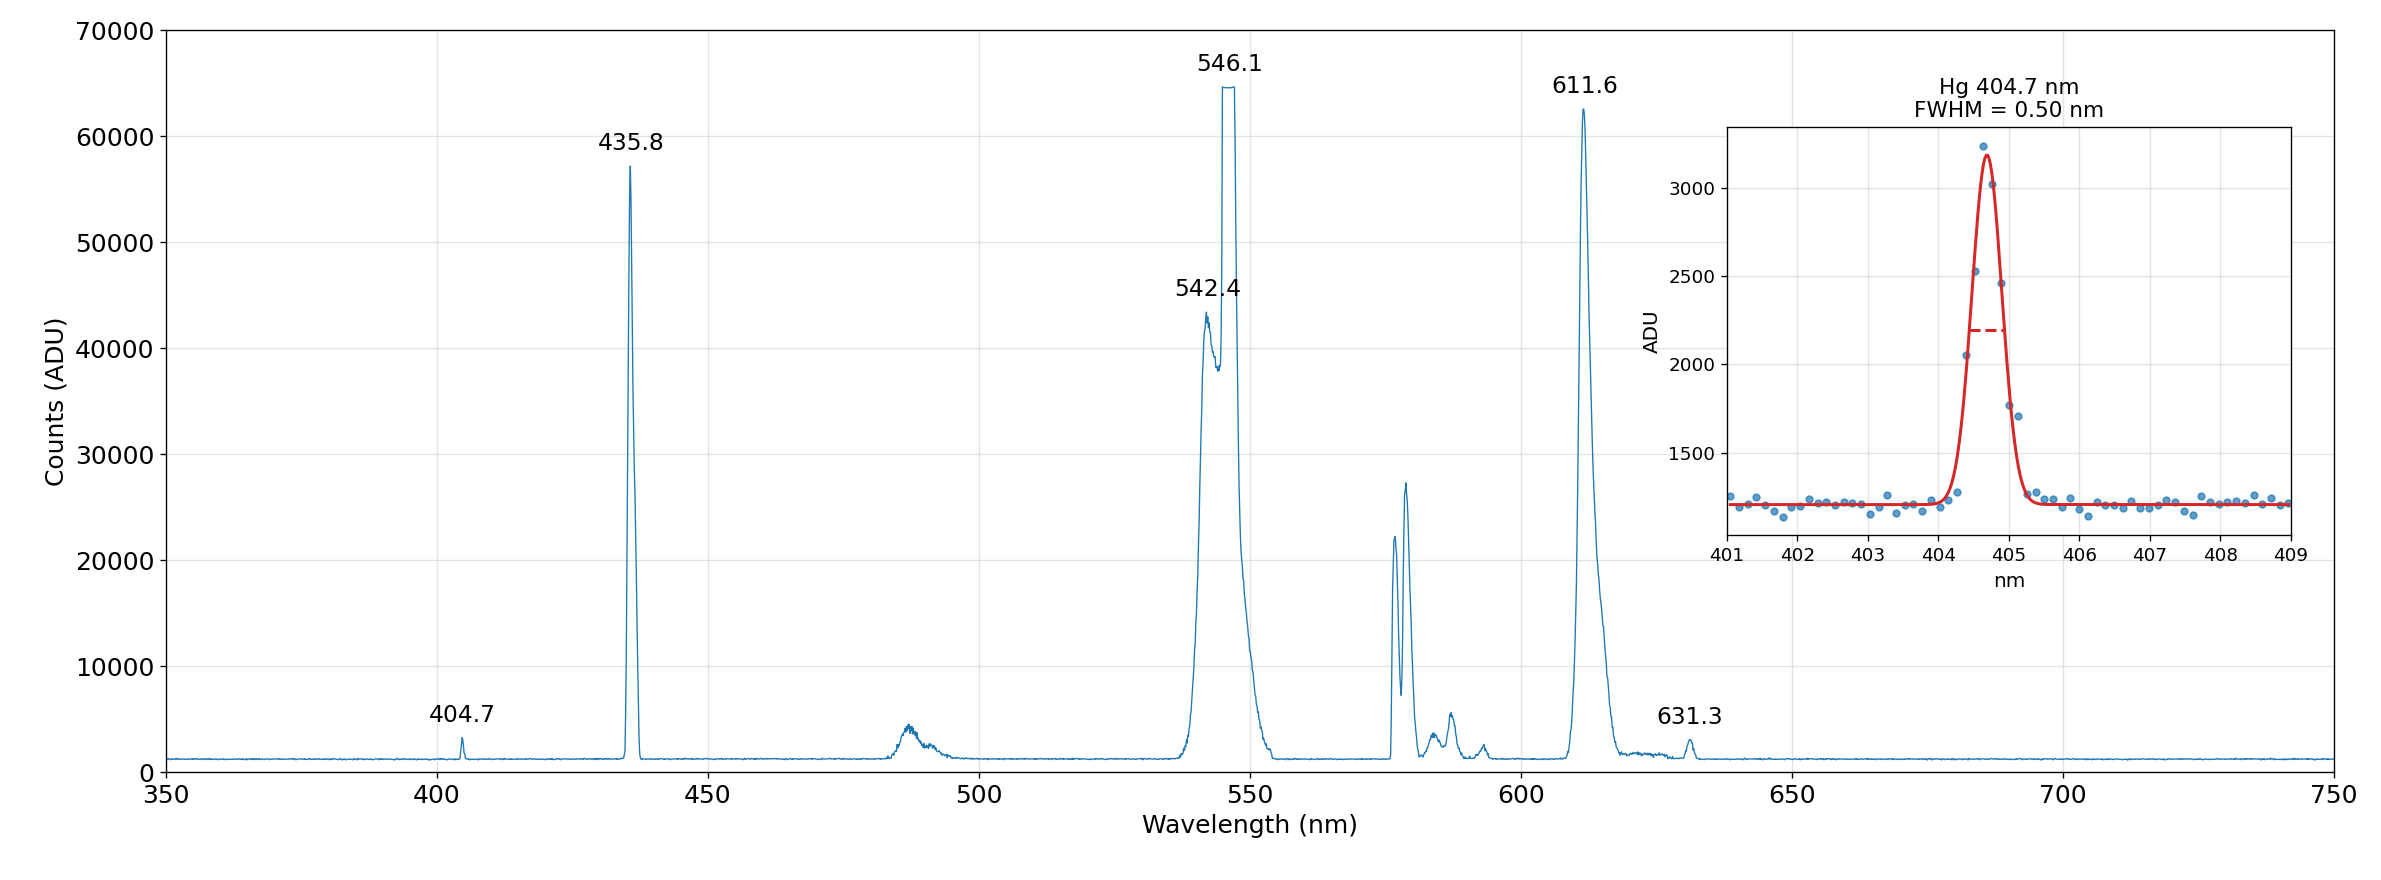
\includegraphics[width=\textwidth]{figures/fig_7_cfl_spectrum.png}
\caption{CFL spectrum captured with the assembled spectrograph.  25\,ms
exposure, single frame, 25\,$\mu$m SMA-905 fiber input.
Inset: Gaussian fit to the Hg\,404.7\,nm line.}
\label{fig:cfl-spectrum}
\end{figure}

\subsection{Summary}

\begin{table}[h!]
\centering
\caption{The v0 design summary.}
\label{tab:v0-summary}
\small
\begin{tabular*}{\textwidth}{@{\extracolsep{\fill}}lllp{4.5cm}@{}}
\toprule
Metric & Target & Achieved & Notes \\
\midrule
Resolution (ILF) & $<$1\,nm EE76 & 0.51--0.85\,nm & 25\,$\mu$m fiber source \\
Spectral range & 400--700\,nm & 350--750\,nm & Grating eff.\ \& mirror refl.\ \\
Spectral coverage & $\geq$300\,nm & 420\,nm & TCD1304 at 14.5\,nm/mm \\
Throughput & $>$0.5\% & 22--41\% & All losses, $\lambda$-dependent \\
$f$-number & $\leq f/4$ & $f/3.9$ & M1: 25.4\,mm, $f{=}100$\,mm \\
RLD & $\leq$17\,nm/mm & 14.5\,nm/mm & 600\,g/mm, $f{=}100$\,mm \\
BOM cost & $<$\$500 & \$904 & \textbf{Exceeds target by 81\%} \\
Full assembly size & --- & 153$\times$168$\times$99\,mm & 3D printed housing \\
\bottomrule
\end{tabular*}
\end{table}

The v0 design meets the resolution target (ILF $<$ 1\,nm) and the
spectral coverage target ($\geq$300\,nm) but misses the BOM cost target.
The primary cost driver is the Thorlabs cylindrical mirrors: M1 and
F1 are \$201 each, accounting for 44\% of the total BOM.  Nevertheless,
every part can be ordered from \texttt{thorlabs.com} with next-day
shipping, making v0 the fastest path to a physical prototype.

\newpage
\clearpage
\phantomsection
\addcontentsline{toc}{section}{References}
\begin{thebibliography}{99}

\bibitem{raysect}
Meakins, A.\ and Carr, M.\ (2014).
Raysect: a ray-tracing framework for scientific simulations.
\url{https://github.com/raysect/source}

\bibitem{tcd1304board}
Nelson, D.R.M.\ (2024).
TCD1304 sensor device with linear response and 16-bit differential
ADC\@.
\url{https://github.com/drmcnelson/TCD1304-Sensor-Device-with-Linear-Response-and-16-Bit-Differential-ADC}

\bibitem{instrcontroller}
Nelson, D.R.M.\ (2025).
Instrumentation controller T4.0 Rev3.
\url{https://github.com/drmcnelson/Instrumentation-Controller-T4.0-Rev3}

\bibitem{s11639board}
Nelson, D.R.M.\ (2024).
S11639-01 linear CCD PCB and code.
\url{https://github.com/drmcnelson/S11639-01-Linear-CCD-PCB-and-Code}

\bibitem{shafer1964}
Shafer, A.B., Megill, L.R., and Droppleman, L.\ (1964).
Optimization of the Czerny-Turner spectrometer.
\textit{Journal of the Optical Society of America}, 54(7), 879--887.

\bibitem{xia2017}
Xia, G., Wu, S., Wang, G., Hu, M., and Xing, J.\ (2017).
Astigmatism-free Czerny-Turner compact spectrometer with
cylindrical mirrors.
\textit{Applied Optics}, 56(32), 9069--9073.

\bibitem{evosolver}
dookaloosy (2026).
evolutionary-solver: domain-agnostic sweep and optimizer engine.
\url{https://github.com/dookaloosy/evolutionary-solver}

\bibitem{build123d}
gumyr (2022).
build123d: a Python CAD programming library built on the OpenCascade
BREP kernel.
\url{https://github.com/gumyr/build123d}

\end{thebibliography}

\end{document}
